\documentclass[]{elsarticle} %review=doublespace preprint=single 5p=2 column
%%% Begin My package additions %%%%%%%%%%%%%%%%%%%
\usepackage[hyphens]{url}

  \journal{?} % Sets Journal name


\usepackage{lineno} % add
\providecommand{\tightlist}{%
  \setlength{\itemsep}{0pt}\setlength{\parskip}{0pt}}

\usepackage{graphicx}
\usepackage{booktabs} % book-quality tables
%%%%%%%%%%%%%%%% end my additions to header

\usepackage[T1]{fontenc}
\usepackage{lmodern}
\usepackage{amssymb,amsmath}
\usepackage{ifxetex,ifluatex}
\usepackage{fixltx2e} % provides \textsubscript
% use upquote if available, for straight quotes in verbatim environments
\IfFileExists{upquote.sty}{\usepackage{upquote}}{}
\ifnum 0\ifxetex 1\fi\ifluatex 1\fi=0 % if pdftex
  \usepackage[utf8]{inputenc}
\else % if luatex or xelatex
  \usepackage{fontspec}
  \ifxetex
    \usepackage{xltxtra,xunicode}
  \fi
  \defaultfontfeatures{Mapping=tex-text,Scale=MatchLowercase}
  \newcommand{\euro}{€}
\fi
% use microtype if available
\IfFileExists{microtype.sty}{\usepackage{microtype}}{}
\usepackage[margin=1.1in]{geometry}
\bibliographystyle{elsarticle-harv}
\usepackage{longtable}
\ifxetex
  \usepackage[setpagesize=false, % page size defined by xetex
              unicode=false, % unicode breaks when used with xetex
              xetex]{hyperref}
\else
  \usepackage[unicode=true]{hyperref}
\fi
\hypersetup{breaklinks=true,
            bookmarks=true,
            pdfauthor={},
            pdftitle={Lethal fox control and fire influence the occurrence of invasive predators and threatened native prey},
            colorlinks=false,
            urlcolor=blue,
            linkcolor=magenta,
            pdfborder={0 0 0}}
\urlstyle{same}  % don't use monospace font for urls

\setcounter{secnumdepth}{5}
% Pandoc toggle for numbering sections (defaults to be off)

% Pandoc citation processing

% Pandoc header
\usepackage{setspace}\doublespacing
\usepackage{float}
\floatplacement{figure}{H}
\newcommand{\beginsupplement}{\setcounter{table}{0}  \renewcommand{\thetable}{S\arabic{table}} \setcounter{figure}{0} \renewcommand{\thefigure}{S\arabic{figure}} \setcounter{section}{0} \renewcommand{\thesection}{S\arabic{section}}}
\usepackage{lineno}
\usepackage{booktabs}
\usepackage{longtable}
\usepackage{array}
\usepackage{multirow}
\usepackage{wrapfig}
\usepackage{float}
\usepackage{colortbl}
\usepackage{pdflscape}
\usepackage{tabu}
\usepackage{threeparttable}
\usepackage{threeparttablex}
\usepackage[normalem]{ulem}
\usepackage{makecell}
\usepackage{xcolor}



\begin{document}
\begin{frontmatter}

  \title{Lethal fox control and fire influence the occurrence of invasive predators and threatened native prey}
    \author[UOM]{Matthew W. Rees\corref{1}}
   \ead{matt.wayne.rees@gmail.com} 
    \author[CEC]{Jack H. Pascoe}
  
    \author[CEC]{Mark Le Pla}
  
    \author[ARI]{Alan Robley}
  
    \author[CEC]{Emma K. Birnbaum}
  
    \author[UOM]{Brendan A. Wintle}
  
    \author[UOM]{Bronwyn A. Hradsky}
  
      \address[UOM]{Quantitative \& Applied Ecology Group, School of Ecosystem and Forest Science, The University of Melbourne, Parkville, VIC, Australia}
    \address[CEC]{Conservation Ecology Centre, Otway Lighthouse Rd, Cape Otway, VIC, Australia}
    \address[ARI]{Department of Environment, Land, Water and Planning, Arthur Rylah Institute for Environmental Research, Heidelberg, Australia}
      \cortext[1]{Corresponding Author}
  
  \begin{abstract}
  
  \end{abstract}
   \begin{keyword} feral cat; diel activity patterns; generalised additive model; invasive predator; intraguild predator interactions; mesopredator release; red fox; lethal predator control\end{keyword}
 \end{frontmatter}

\parskip=12pt

\emph{Article type}: Research Article

\emph{Running title}: XX

\emph{Word count (abstract, body)}: XX, XX

\emph{References}: ?

\emph{Figures}: 5

\emph{Tables}: 0

\emph{Authorship}:

\emph{Data accessibility}: Data and code will be deposited on the Dryad Digital Repository after acceptance and can be viewed here: \url{https://github.com/matt-w-rees/sw-vic-occurrence-phd}.

\newpage

\hypertarget{abstract}{%
\section*{ABSTRACT}\label{abstract}}
\addcontentsline{toc}{section}{ABSTRACT}

Invasive predators and altered fire regimes are key, often overlapping biodiversity threats. Disentangling the impacts of multiple threats and management actions is challenging, particularly when species occur patchily across heterogeneous landscapes.

Here we assessed the effects of lethal control of an introduced apex predator, the red fox \emph{Vulpes vulpes}, on mammal communities in fire-prone and fragmented forests of south-eastern Australia. Our study synthesised data from multiple smaller-scale studies that used a combination of experimental and space-for-time approaches to monitor the effects of fox control and time since fire on mammals, giving a total of 3667 camera-traps deployments across 1232 sites (172,052 trap nights). We used occupancy-detection models to investigate species detectability, and generalised additive models to explore potentially nonlinear effects of multiple drivers and management actions on the distribution of two invasive mammalian predators and two threatened native prey species.

In one region with frequent, long-term (8 - 14 years) targeted poison-baiting of foxes, foxes were heavily suppressed in terms of both detectability and occupancy. There was some evidence feral cat \emph{Felis catus} occupancy was slightly higher in landscapes with fox control, potentially signalling mesopredator release. Among the threatened native prey species, occupancy rates of long-nosed potoroos \emph{Potorous tridactylus} were higher in landscapes with fox control, but there was little difference in southern brown bandicoot \emph{Isoodon obesulus} occupancy. In another region where fox control recently commenced (0 - 2 years), foxes were suppressed to a lesser extent, and no impacts were detected on subordinate predator or prey species. Fire history impacted the occurrence of each study species; however, invasive predators responded differently to time since fire (0 - 80 years) across each vegetation type.

Predator control and prescribed fire are important and widely used management tools. The conservation benefits of introduced depend on the intensity and duration of management, and optimal fire regimes differ between species and vegetation types.

\newpage

\hypertarget{introduction}{%
\section{INTRODUCTION}\label{introduction}}

Accurate and precise estimates of the effects of management are essential to inform conservation decision-making, ensure cost-effective allocation of resources and identify potential unintended consequences of interventions (Christie \emph{et al.} 2020). However, reliable inference about the effects of landscape-scale management, including identifying the cause of nil or perverse outcomes, is often difficult to achieve because target populations fluctuate naturally and are often subject to multiple co-occurring threats and management actions (Pressey \emph{et al.} 2007; Sugihara \emph{et al.} 2012). Separating management effects from other drivers is particularly difficult for species that occur patchily across broad distributions (Tulloch \emph{et al.} 2016).

Invasive predator management is a classic example of these challenges. Predators can have devastating impacts on native biodiversity when introduced beyond their native range, and so invasive predators are often actively controlled using lethal methods (Sih \emph{et al.} 2010; Bellard, Genovesi, \& Jeschke 2016; Doherty \emph{et al.} 2016). Quantifying the degree of invasive predator suppression, the responses of their native prey and any unintended outcomes across gradients of predator control is key to designing effective, cost-efficient management programs (Baxter \emph{et al.} 2008; Walsh \emph{et al.} 2012; Cattarino \emph{et al.} 2016). However, the ability of associated monitoring programs to detect these signals is often limited by confounding from co-occurring threats, management actions and natural drivers. This is concerning because, in many cases, few or negative effects on native biodiversity are observed following invasive predator control, particularly when multiple introduced species are present (Ballari, Kuebbing, \& Nuñez 2016).

There are several explanations for why native prey species may not benefit from invasive predator control. Firstly, control efforts may not sufficiently reduce the density of invasive predators---predators can be remarkably resilient to low-effort culling (Sinclair \emph{et al.} 1998; Sabo 2005; Lazenby, Mooney, \& Dickman 2015; Moseby \emph{et al.} 2019). Secondly, invasive predator suppression may lead to a `release' of a subordinate predator (Courchamp, Langlais, \& Sugihara 1999; Crooks \& Soulé 1999) or competitor species (Ruscoe \emph{et al.} 2011), which could potentially worsen net outcomes for the native species (e.g., Rayner \emph{et al.} 2007). Thirdly, predation by introduced species may not be the primary limit on native prey populations (Banks 1999). Hence, quantifying the degree of apex predator suppression and testing the mesopredator release hypothesis (Prugh \emph{et al.} 2009), are important steps toward understanding prey responses to lethal predator control and identifying the cause of a nil response, if observed.

Quantifying the impacts of planned fire on fauna is similarly complex. Fire can drive the persistence and abundance of fauna populations, primarily through its effects of vegetation structure (Monamy \& Fox 2000). As these effects persist for decades or centuries, are nonlinear, and vary across environmental conditions (Haslem \emph{et al.} 2011), fauna species' responses to fire often vary across heterogeneous landscapes (Nimmo \emph{et al.} 2014; Swan \emph{et al.} 2015). Predicting the long-term ramifications of fire for predators and prey is a key challenge for managers who are tasked with stemming the decline of native fauna populations while simultaneously managing fuel loads to protect against the increasing threat of large wildfires (Clarke 2008; Hradsky 2020).

These separate challenges are amplified in contexts where invasive predators occur in fire-prone landscapes (Doherty \emph{et al.} 2015). Nonetheless, disentangling the complex and potentially interacting effects of invasive predator and fire management on threatened native fauna is crucial for effective native mammal conservation in Australia, which has experienced some of the worst biodiversity declines in recent world history (Waldron \emph{et al.} 2017; Woinarski \emph{et al.} 2019). Predation by introduced species and altered fire regimes are primary drivers of these declines (Woinarski, Burbidge, \& Harrison 2015), but other threatening processes such as habitat fragmentation, and natural drivers such vegetation type and rainfall dynamics also play an important role in shaping contemporary native mammal distributions (May \& Norton 1996; Hale \emph{et al.} 2016). Lethal red fox \emph{Vulpes vulpes} (hereafter `fox') control and prescribed burning (primarily for asset protection) are among the most common management actions in protected areas, however, we have a poor understanding of their effects on native fauna (Clarke 2008; McLeod \emph{et al.} 2008; Braysher 2017; Lindenmayer \emph{et al.} 2018; Hradsky 2020). This is partly because there is strong spatial overlap of these threats and management actions (Evans \emph{et al.} 2011) and potential unintended consequences often go unmeasured.

In this study, we assessed the effect of landscape-scale lethal fox management in two protected, fire-prone conservation regions of south-eastern Australia: the Glenelg region and Otway Ranges. We quantified the effects of fox management on foxes (the managed species), feral cats \emph{Felis catus} (hereafter `cat'; unmanaged competitor), and two threatened species that are the primary focus of the conservation programs: the southern brown bandicoot \emph{Isoodon obesulus} (hereafter `SBB') and long-nosed potoroo \emph{Potorous tridactylus} (hereafter `LNP'). Our study dataset combined experimental and space-for-time approaches through one-off and repeat deployments of 3667 camera-traps across 1232 sites over a period of seven years. In the Glenelg region, foxes had been continuously controlled for 8 - 14 years; In the Otway region, we examined the effects of a new fox control program over a 3 year period; both regions also included substantial unbaited areas as experimental controls. Occupancy-detection models (MacKenzie \emph{et al.} 2002) were used to investigate the detectability of each species. As detectability was generally high, we then used Generalised Additive Models (hereafter `GAMs'; Wood 2017) to explore the potentially nonlinear responses of each species to fox control effort (1080 poison-bait density), time since fire (0 - 80 years) across vegetation types, and other environmental drivers (elevation, terrain ruggedness, recent rainfall, topographic wetness and habitat fragmentation). The GAMs did not account for imperfect detection, but allowed nonlinear responses and more complex model structures.

\newpage

\hypertarget{materials-and-methods}{%
\section{MATERIALS AND METHODS}\label{materials-and-methods}}

\hypertarget{study-regions}{%
\subsection{Study regions}\label{study-regions}}

We compiled data from multiple camera-trap studies across two regions in south-west Victoria, Australia: the Glenelg region and Otway Ranges (Fig. \ref{fig:occ-map}). Introduced foxes and cats are the only medium-large functional mammalian terrestrial carnivores here: native dingoes \emph{Canis familiaris} are long-absent throughout, while tiger quolls \emph{Dasyurus maculatus} are long-absent in the Glenelg region and likely functionally extinct in the Otway Ranges (last confirmed sighting in 2014). Managers frequently implement prescribed fire across both regions, primarily to reduce fuel loads.

\hypertarget{glenelg-region}{%
\subsubsection{Glenelg region}\label{glenelg-region}}

In the Glenelg region (38°05'54``S 141°44'41''E), large patches of natural vegetation are fragmented mostly by pastoral farming and residential properties (Fig. \ref{fig:occ-map}). Here, the primary vegetation communities are heathy woodland, lowland forest, herb-rich woodland and wet heathland (Department of Environment, Land, Water \& Planning 2020a). The Glenelg region has an annual mean minimum temperature of 8.1 °C in winter, and 20.0 °C in Summer (Bureau of Meteorology 2021). Mean annual rainfall averages 835 mm (Bureau of Meteorology 2021). Terrain is gently undulating in the Glenelg region; study sites ranged from 12 - 180 m above sea level.

\hypertarget{otway-ranges}{%
\subsubsection{Otway Ranges}\label{otway-ranges}}

The Otway Ranges (38°57'82``S 141°68'41''E) is a largely continuous patch of natural vegetation with a strong east-west rainfall gradient (Fig. \ref{fig:occ-map}). A matrix of cool temperate rainforest and wet forest at high-altitudes in the south-west descend into a large heathland directly north, and into dry forests and then heathlands to the north-east. Annual rainfall averages 1955 mm in the southwest, dropping to 627 mm in the eastern Otways (Bureau of Meteorology 2021). Mean minimum temperatures in the Otway Ranges are 8° in winter and 13° in summer (Bureau of Meteorology 2021). Our study sites ranged from 23 - 617 m above sea level.

\hypertarget{fox-control-and-monitoring}{%
\subsection{Fox control and monitoring}\label{fox-control-and-monitoring}}

In broad sections of each region, government land managers conduct ongoing targeted lethal fox control for biodiversity conservation. Poison-baits containing 3 mg of sodium mono-fluroacetate (`1080') are buried at a depth of 12 - 15 cm at 1-km intervals along accessible forest tracks and roads. Different road densities result in spatially variable densities of poison-baits.

\hypertarget{glenelg-region-1}{%
\subsubsection{Glenelg region}\label{glenelg-region-1}}

In the Glenelg region, three distinct forest blocks have been subject to poison-baiting since October 2005, with fortnightly bait replacements. These forest blocks, along with three similar, unbaited forest blocks to the north are simultaneously surveyed annually under the `Glenelg Ark' fox control program (40 camera-sites per block; Robley \emph{et al.} 2020). Hair-tubes were used to monitor small prey species from 2005 - 2013 (presented in Robley \emph{et al.} 2014), replaced by camera-traps from 2013 onwards (here we present camera-trap data from 2013 - 2019; Robley \emph{et al.} 2020). We also included a further 425 camera-trap deployments at unique locations from early 2018 (M.W.R., PhD surveys). This totals 2041 camera-trap deployments in the Glenelg region, collected in a control-impact experimental design (foxes had been continuously controlled for at 8 - 14 years in the treatment landscapes by the time of these surveys).

\hypertarget{otway-ranges-1}{%
\subsubsection{Otway Ranges}\label{otway-ranges-1}}

Fox-baiting commenced in small sections of the Otway Ranges in 2008 and large-scale systematic baiting began in 2016 - 2017 under the `Otway Ark' program (Robley, Moloney, \& Parks Victoria West Coast District Team 2019). For the first six weeks of the Otway Ark program, poison-baits were replaced weekly, this then changed to ongoing monthly bait-replacement. There was a pause in baiting for approximately six months during the second half of 2018. Fox control recommenced in late 2018 with four weeks of fortnightly bait-replacement, before returning to monthly bait-replacement. A large section of the Otway Ranges to the north-west remains unbaited, but is monitored as an experimental non-treatment site (Robley, Moloney, \& Parks Victoria West Coast District Team 2019). Otway Ark managers survey 372 camera-trap sites annually (sequentially across the region); we present one `before' baiting survey and two `after' baiting surveys of each site from 2016 - 2018, totalling 1113 camera-trap deployments (Robley, Moloney, \& Parks Victoria West Coast District Team 2019). We also include data from an additional before-after control-impact surveys (one `before' baiting survey and two `after' bating surveys) in the western section of the Otway Ranges, conducted annually 2017 - 2019 (M.W.R PhD surveys). This added a further 195 sites and 513 camera-trap deployments.

\hypertarget{camera-trap-set-ups}{%
\subsubsection{Camera-trap set-ups}\label{camera-trap-set-ups}}

All camera-trap deployments consisted of a Reconyx (Holmen, Wisconsin) brand camera-trap (white or infrared flash), attached to a tree or a metal picket, facing a lure. The Glenelg Ark and Otway Ark fox monitoring programs positioned camera-traps at least 40 cm above ground on a tree or a metal picket, angled downwards toward a lure approximately 1 - 1.5 m away (Robley, Moloney, \& Parks Victoria West Coast District Team 2019; Robley \emph{et al.} 2020). The lure consisted of peanut butter, golden syrup and rolled oats mixed into a small ball, placed within a tea strainer or PVC pipe container and secured either to the ground, or 20 - 60 cm above ground on a wooden stake. The M.W.R. PhD surveys across both regions positioned camera-traps lower on a tree (around 15 - 30 cm above the ground) angled only slightly downwards towards a tuna oil lure approximately 2 - 2.5 m away (detailed in Rees \emph{et al.} 2019). Camera-traps were active for an average of 47 days (maximum 93 days), totalling 172,052 trap-nights. Camera-traps that were active for fewer than ten days were discarded from the dataset.

\hypertarget{study-species}{%
\subsubsection{Study species}\label{study-species}}

Foxes and feral cats are both introduced to Australia and share a similar functional niche (Glen \& Dickman 2005), competing for many of the same prey species (Stobo-Wilson \emph{et al.} 2021a; b; Woinarski \emph{et al.} 2021). The two threatened prey species, LNPs and SBBs are both solitary, medium-sized, ground-dwelling marsupials. They nest in dense understorey vegetation during the day and turn over large quantities of soil to feed on invertebrates, plant material and fungi at night (Van Dyck \& Strahan 2008).

\hypertarget{occupancy-detection-models}{%
\subsection{Occupancy-detection models}\label{occupancy-detection-models}}

We first modelled species occupancy probabilities using occupancy-detection models (MacKenzie \emph{et al.} 2002) implemented in a Bayesian framework using `stan' (Carpenter \emph{et al.} 2017) via the `ubms' R-package (Kellner 2021). For each species, we fit a `stacked' single-season model: repeat surveys were considered as additional sites and pseudoreplication accounted for by using a random-intercept for each unique site. We defined survey occasions as 24-hour periods commencing at midday. We modelled the effect of fox control (categorical: baited or unbaited) on species occupancy and detectability, and included an interaction term with region to account for potentially different responses in the Glenelg and Otway regions. We fit models with four MCMC chains each with 10,000 iterations (including a 5000-iteration warm-up phase). To determine whether species detection probabilities were high enough to permit analysis with generalised additive models (which do not account for imperfect detection), we calculated cumulative detection probabilities for camera-trap survey lengths (Garrard \emph{et al.} 2008) from one to 93 days (maximum survey duration).

\hypertarget{generalised-additive-models}{%
\subsection{Generalised Additive Models}\label{generalised-additive-models}}

The occupancy-detection models revealed high (\textgreater{} 75\%) cumulative detection probabilities for each species across baited and unbaited landscapes for each region, based on our average camera-trap survey effort, except for cats in the Glenelg region (see results for details). We therefore went on to model species occurrence probabilities using binomial GAMs implemented in the `mgcv' R-package (Wood 2017). The use of GAMS has the advantage of allowing modelling of non-parametric and nonlinear relationships between response (species occurrence) and explanatory variables (particularly important for estimating time since fire responses; Haslem \emph{et al.} 2011) in a computationally efficient framework.

The response variable in the GAMs was binary occupied-unoccupied for each species for the entire camera-trap deployment. To account for differences in survey duration, we specified a model offset for the log-transformed survey duration (number of days); we also included a random intercept for each unique camera-site to account for repeat sampling. We used the double penalty model selection approach, which penalises model complexity both in terms of the model structure (explanatory variables included) and the shape (wiggliness) of the relationships between the responses and explanatory variables (Marra \& Wood 2011). We used the same model structure for each species, as detailed in the sections below. We assessed model fits (proportion of the null deviance explained, adjusted R-squared value) and predictive performance measures (Akaike Information Criterion score; hereafter `AIC'; Burnham \& Anderson 2004) against a `null model' for each species which only had a random intercept for each camera site.

\hypertarget{poison-bait-density}{%
\subsubsection{1080 poison-bait density}\label{poison-bait-density}}

Poison-baits are deployed by land managers to suppress foxes with the aim of benefiting native prey. The degree of fox suppression is likely to be a function of the spatial arrangement of poison baits (i.e., poison-bait density) relative to fox home-range size, as well as the frequency of bait replacement (Fleming 1996; Benshemesh \emph{et al.} 2020). In the Otway and Glenelg regions, adult foxes travel an average maximum distance of 2.3 km from their home-range centre (Hradsky \emph{et al.} 2017b). Therefore, to examine the typical lethal control effort experienced by a fox in these landscapes, we summed the number of poison-bait stations within a 2.3 km radius around each camera-trap deployment. Bait densities ranged from 0 - 19 baits per 16.1 km\textsuperscript{2} circle (2.3 km radius), with a mean value of 10 and eight baits per circle in fox-baited landscapes in the Glenelg region and Otway Ranges, respectively. For an easier comparison to other studies, we converted these values to baits per square kilometre. We modelled a function of 1080 poison-bait density with separate responses per region. Interpretation of these relationships should keep in mind that they are context-specific and do not account for the fact that (i) in wet weather conditions, some poison-bait stations become inaccessible and baits do not get replaced, or (ii) there was an approximate six month pause in bait replacements in the Otway Ranges in 2018.

\hypertarget{fire-and-vegetation-type}{%
\subsubsection{Fire and vegetation type}\label{fire-and-vegetation-type}}

We expected species occurrence to (i) differ across vegetation types, (ii) respond to TSF, and (iii) have variable responses to TSF in each vegetation type (as post-fire regeneration occurs at different speeds; Swan \emph{et al.} 2015). We also expected species to respond to fire frequency, as this can have a strong effect on vegetation structure (Collins \emph{et al.} 2012).

We derived fire frequency (the number of previous fires) and time since last fire (in years) for each camera trap deployment using coarse fire scar mapping provided by government managers, dating back to 1939 when large wildfires burnt both regions extensively. On average, sites for each camera-trap deployment had been burnt 1.5 times since 1939 at the time of camera deployment. The most frequently burnt sites (two deployments at different unique sites) had experienced eight fires; 397 camera-trap deployments (11\%) had not burnt since 1939. We identified the Ecological Vegetation Class group (hereafter `vegetation type'; standard units for vegetation classification in Victoria; Department of Environment, Land, Water \& Planning 2020a) for each unique camera-trap site, totalling eight vegetation types. We only surveyed 20 unique sites in rainforests, which are interspersed (primarily in low lying gullies) throughout wet and damp forests in the south-eastern Otway Ranges. Given the similarity, fine-scale interspersion of these EVC groups, and that both rarely or never experience fire, we merged them together (hereafter referred to as `wet forests').

We modelled an interaction between time since fire (in years; hereafter `TSF') and vegetation type by using a hierarchical model structure, which estimated an average TSF response for each species, along with separate responses to TSF in each vegetation type (model `GS' detailed in Pedersen \emph{et al.} 2019). This approach shares information on TSF responses and wiggliness across EVC groups, penalising functions which deviate strongly from the average response that are not substantially supported by the observation data. We initially fit a separate smooth for fire frequency, however, this had high concurvity with TSF (causing a lack of identifiability) and so we removed the fire frequency variable from all models.

\hypertarget{elevation-topographic-ruggedness-and-wetness}{%
\subsubsection{Elevation, topographic ruggedness and wetness}\label{elevation-topographic-ruggedness-and-wetness}}

Elevation is a strong driver of rainfall, moisture and temperature gradients in both regions, likely indirectly impacting the distribution of the study species through resource availability. High topographic complexity (i.e., `ruggedness') can limit predator movement and predation rates, thereby benefiting prey (McKenzie \emph{et al.} 2007; Hohnen \emph{et al.} 2016; McDonald \emph{et al.} 2017; Stobo-Wilson \emph{et al.} 2020b). Soil moisture (estimated by the topographic wetness index) impacts vegetation, as well as the availability of subterranean invertebrates and fungi - key food sources for LNPs and SBBs (Lobert 1990; Nuske \emph{et al.} 2017).

We extracted the elevation above sea level (metres) of each site using a 10-m resolution digital elevation model (Department of Environment, Land, Water \& Planning 2020b). We also used this elevation layer to calculate the median terrain ruggedness index (calculates the difference in elevation between a central cell and eight adjacent cells; Riley, DeGloria, \& Elliot 1999), taking the median value in a 30-m radius around each camera-trap site. The topographic wetness index estimates where water will accumulate by accounting for topographic influences on hydrological processes (Beven \& Kirkby 1979). We also took the median topographic wetness index in a 30-m radius around each camera-trap site, derived from a 30-m resolution layer (Gallant \& Austin 2012). We modelled the effect of elevation, as well as indices of topographic ruggedness and wetness (both derived from a digital elevation model) on species occurrences.

\hypertarget{proximity-to-forest-edge}{%
\subsubsection{Proximity to forest edge}\label{proximity-to-forest-edge}}

Invasive predators are well-documented to prefer edges between forest and cleared land as they facilitate efficient movement and hunting (e.g., Hradsky \emph{et al.} 2017b; McGregor \emph{et al.} 2014; Nichols \emph{et al.} 2019). We modelled the effect of the minimum distance from each camera-trap site to the nearest substantial area of non-native vegetation. We calculated this by inverting the extent of native vegetation (Department of Environment, Land, Water \& Planning 2019) and removing cleared areas smaller than 30 ha, as per Geary \emph{et al.} (2020).

\hypertarget{recent-rainfall}{%
\subsubsection{Recent rainfall}\label{recent-rainfall}}

Changes in short-term rainfall dynamics likely impact invasive predator and native prey species (Arthur, Catling, \& Reid 2012; Wilson \emph{et al.} 2012; Paull, Mills, \& Claridge 2013; Greenville \emph{et al.} 2014). We therefore calculated the percentage difference in rainfall from the long-term median that had occurred prior to the start of each camera-trap deployment in a six, 12, 18 and 24 month period. We used rainfall data from the nearest weather station (n = 11; Bureau of Meteorology 2021) for each camera-trap. We modelled rainfall effects separately for each region. To identify the most appropriate rainfall window (six -- 24 months) for each species, we fit a separate model (including all other explanatory variables listed above) using each rainfall window and selected the top-ranked model using AIC scores.

All analyses were conducted in R version 3.6.3 (R Core Team 2020).

\newpage

\begin{figure}

{\centering 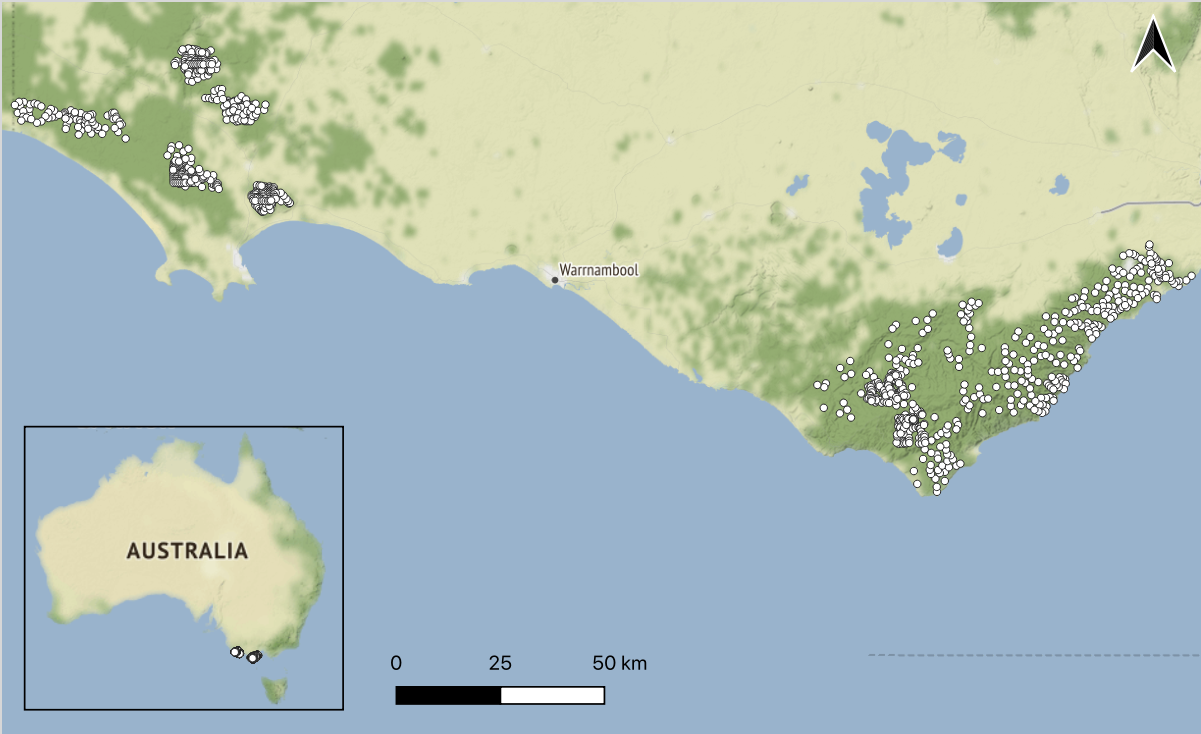
\includegraphics[width=0.8\linewidth]{../figs/map_cams} 

}

\caption{Locations of our study regions in south-west Victoria, Australia. The grids of camera-traps are denoted by white dots. The Glenelg region is to the west and Otway region to the east. Native vegetation is indicated by dark green, with hill shading. \textit{Map tiles by Stamen Design, under CC BY 3.0, map data by OpenStreetMap, under CC BY SA.}}\label{fig:occ-map}
\end{figure}

\newpage

\hypertarget{results}{%
\section{RESULTS}\label{results}}

\hypertarget{red-fox}{%
\subsection{Red fox}\label{red-fox}}

Foxes were detected on 1453 of the 3667 camera-traps surveys (39.6\%; Table \ref{tab:occ-naive}).

\hypertarget{occupancy-detection-models-1}{%
\subsubsection{Occupancy-detection models}\label{occupancy-detection-models-1}}

Fox detectability in unbaited landscapes was high, particularly in the Glenelg region (Fig. \ref{fig:occ-det}a) where 95\% detection probability was reached after a 30 day survey duration (relative to 64 days in the Otway Ranges; Fig. \ref{fig:occ-cumdet}). Fox control reduced fox detectability across both regions. Nonetheless, foxes in baited landscapes still had a high detection probability for the average survey duration (47 days): 76\% in the Glenelg region and 81\% in the Otway Ranges (Fig. \ref{fig:occ-cumdet}).

The occupancy-detection model estimated fox occupancy to be lower at sites in baited landscapes than unbaited landscapes; this effect was more than twice as strong in the Glenelg region than the Otway Ranges (Fig. \ref{fig:occ-det}b). For example, in heathy woodlands of the Glenelg region, fox occupancy probability was approximately three times lower in baited landscapes (0.19; 95\% CI 0.13 - 0.26) relative to unbaited landscapes (0.56; 95\% CI: 0.47 - 0.66). Whereas in the heathy woodlands of the Otway Ranges, fox occupancy was already low without fox control (0.33; 95\% CI: 0.25 - 0.43) and was approximately 1.4 times lower following fox control (0.24; 95\% CI 0.17 - 0.33). Foxes were ubiquitous across the study regions, but the probability of occupancy was nearly twice as high in dry forests, herb-rich woodlands and lowland forests than heathlands, heathy woodlands and wet forests (Fig. \ref{fig:occ-det}c).

\hypertarget{generalised-additive-models-1}{%
\subsubsection{Generalised additive models}\label{generalised-additive-models-1}}

The GAM showed that fox-bait density in the Glenelg region was the strongest driver of fox occurrence. Fox occurrence in the Glenelg region declined from a probability of 0.68 (95\% CI: 0.58 - 0.76) where fox-bait density was zero, to 0.04 (95\% CI: 0.02 - 0.11) where fox-bait density was highest (1.14 baits km\textsuperscript{-2}; Fig. \ref{fig:gams-occ-fox}a). The effect of fox-bait density on foxes in the Glenelg region was nonlinear: there was little difference in fox occurrence across the range of 0.4 to 0.8 baits km\textsuperscript{-2}, but a greater suppression was achieved at higher bait densities (Fig. \ref{fig:gams-occ-fox}a). Fox occurrence also declined with fox-bait density in the Otway Ranges, but this effect was linear, weaker and had higher uncertainty (Fig. \ref{fig:gams-occ-fox}a). In the Otway Ranges, fox occurrence declined from a probability of 0.4 (95\% CI: 0.32 - 0.48) where fox-bait density was zero, to 0.14 (95\% CI: 0.05 - 0.35) where fox-bait density was highest (1.1 baits km\textsuperscript{-2}; Fig. \ref{fig:gams-occ-fox}a).

There was no average TSF response on fox occurrence, however, fox occurrence declined linearly with TSF in dry forests and increased linearly with TSF in heathland, although there was considerable uncertainty in these estimates (Fig. \ref{fig:gams-occ-fox}g:h).

Fox occurrence declined linearly with increasing terrain ruggedness, and with distance to non-native vegetation for distances up to approximately 1.5 - 2 km (Fig. \ref{fig:gams-occ-fox}d;f). Elevation had a nonlinear and uncertain effect on fox occurrence, which was estimated to peak around 450 m above sea level (Fig. \ref{fig:gams-occ-fox}c). The effect of topographic wetness on fox occurrence was removed from the model (Fig. \ref{fig:gams-occ-fox}e). The fox GAM that considered rainfall deviations in the previous 6 months was ranked highest relative to models with 18- (by only 1.4 AIC units), 12-, and 24-month periods (by at least 6.4 AIC units; Table. \ref{tab:occ-rain-aic}; however, this effect was weak with relatively high uncertainty (Fig. \ref{fig:gams-occ-fox}c).

The top-ranked fox GAM had an adjusted R-square value of 0.27 and explained 26\% of the null deviance. Relative to the null model (with only a site random intercept), the explanatory variables improved predictive performance considerably (242 AIC units lower), but slightly worsened the model fit (Table. \ref{tab:occ-model-sumstats}).

\hypertarget{feral-cat}{%
\subsection{Feral cat}\label{feral-cat}}

Cats were detected on 1010 camera-trap deployments (27.6\%; Table \ref{tab:occ-naive}).

\hypertarget{occupancy-detection-models-2}{%
\subsubsection{Occupancy-detection models}\label{occupancy-detection-models-2}}

Cats were relatively poorly detected in the Glenelg region, where they had a 59\% detection probability given presence for the average survey duration, compared to 83\% in the Otway Ranges; Fig. \ref{fig:occ-cumdet}). There was no detectability difference between fox control treatment landscapes in the Glenelg region, however, cat detectability was slightly higher with fox control in the Otway Ranges (Fig. \ref{fig:occ-det}a).

The occupancy-detection models estimated that cat occupancy in the Glenelg region was higher in landscapes with fox control (e.g., 0.25 in heathy woodlands; 95\% CI: 0.16 - 0.35 in heathy woodlands) relative to those without fox control (0.12 in heathy woodlands; 95\% CI: 0.07 - 0.19); but there was no association with baiting in the Otway Ranges (Fig. \ref{fig:occ-det}b). Cat occupancy was most strongly driven by vegetation type: highest in the wet forest, followed by heathland, swampy scrub, herb-rich woodland and dry forest, but very low in lowland forest and heathy woodland (Fig. \ref{fig:occ-det}c).

\hypertarget{generalised-additive-models-2}{%
\subsubsection{Generalised additive models}\label{generalised-additive-models-2}}

The cat GAM showed no effect of fox-bait density, elevation or topographic wetness on cat occurrence (Fig. \ref{fig:gams-occ-cat}a;c;e). Cats responded to TSF differently across each vegetation type, with the average TSF response removed from the model (Fig. \ref{fig:gams-occ-cat}g:h). Cat occurrence probability increased with terrain ruggedness, and declined with distance from the nearest area of non-native vegetation, although uncertainty was high (Fig. \ref{fig:gams-occ-cat}d;f). The different rainfall deviation windows were were indistinguishable based on AIC scores; but in all cases except 6 months, the rainfall variable was removed from the model. The model that considered rainfall deviations in the previous six months was marginally top-ranked (by 0.7 AIC units) and estimated that cat occurrence slightly increased as rainfall increased (relative to the long-term average; Fig. \ref{fig:gams-occ-cat}c).

The top-ranked cat GAM had an adjusted R-square value of 0.24 and explained 24\% of the null deviance. Relative to the null model, the explanatory variables improved predictive performance considerably (168 AIC units lower), but only slightly improved the model fit (less than 1\% increase in null deviance explained and 0.02 for the R-squared value; Table. \ref{tab:occ-model-sumstats}).

\hypertarget{southern-brown-bandicoot}{%
\subsection{Southern brown bandicoot}\label{southern-brown-bandicoot}}

We detected SBBs on 394 of the 3667 camera-traps (10.7\%; Table \ref{tab:occ-naive}).

\hypertarget{occupancy-detection-models-3}{%
\paragraph{Occupancy-detection models}\label{occupancy-detection-models-3}}

SBBs were highly detectable, with a greater than 95\% detection probability reached after 31 and 43 days in the Glenelg and Otway Ranges, respectively (Fig. \ref{fig:occ-cumdet}). Baiting was associated with a decrease in SBB detectability in Glenelg but an increase in detectability in the Otways (Fig. \ref{fig:occ-det}a).

There was no discernible effect of fox control on SBB occupancy in either region (Fig. \ref{fig:occ-det}b). SBB's were most likely to occupy heathy woodlands (Fig. \ref{fig:occ-det}c) and they were largely absent from the wet forests (Table \ref{tab:occ-naive}). The few SBB detections in wet forest occurred at sites adjacent to other vegetation types (SBBs are largely replaced by long-nosed bandicoots \emph{Perameles nasuta} in wet forest; M. Rees, unpublished data).

\hypertarget{generalised-additive-models-3}{%
\subsubsection{Generalised additive models}\label{generalised-additive-models-3}}

SBB occurrence probability was very low. There was some indication SBB occurrence slightly increased with fox-bait density in the Glenelg region, peaking at around 150 m above sea level and 2 km from the nearest forest edge and declined with increasing terrain ruggedness and TSF; however, these explanatory variables had high uncertainty relative to the strength of the effects (Fig. \ref{fig:gams-occ-sbb}). There was no evidence that rainfall affected SBB occurrence -- the top-ranked models in terms of AIC scores (Table. \ref{tab:occ-rain-aic}) had the effects of rainfall completely removed.

The top-ranked SBB GAMs had an adjusted R-square value of 0.31 and explained 41\% of the null deviance. Relative to the null model, the explanatory variables improved predictive performance considerably (211 AIC units lower) and slightly improved the model fit by 4\% of null deviance explained and 0.05 for the R-squared value (Table. \ref{tab:occ-model-sumstats}).

\hypertarget{long-nosed-potoroo}{%
\subsection{Long-nosed potoroo}\label{long-nosed-potoroo}}

We detected LNPs on 331 camera-trap deployments (9\%; Table \ref{tab:occ-naive}).

\hypertarget{occupancy-detection-models-4}{%
\subsubsection{Occupancy-detection models}\label{occupancy-detection-models-4}}

LNPs were the most detectable of our study species, reaching a 95\% detection probability with a 33 and 18 day survey duration in the unbaited landscapes of the Glenelg and Otway regions, respectively (Fig. \ref{fig:occ-cumdet}). In the Glenelg region, LNP detectability was twice as high in landscapes with fox control relative to those without (Fig. \ref{fig:occ-det}a). Occupancy of LNPs was highest in heathlands (Fig. \ref{fig:occ-det}c).

\hypertarget{generalised-additive-models-4}{%
\subsubsection{Generalised additive models}\label{generalised-additive-models-4}}

The GAM showed that LNP occupancy improved from a 0.05 probability (95\% CI: 0.02 - 0.11) to 0.33 (95\% CI: 0.16 - 0.55) across the fox-bait density gradient in the Glenelg region (Fig. \ref{fig:gams-occ-lnp}a). In contrast, LNP occupancy showed no relationship with poison-bait density in the Otway region (Fig. \ref{fig:gams-occ-lnp}a). LNP occurrence probability increased linearly with elevation (Fig. \ref{fig:gams-occ-lnp}c) and peaked in the mid-range of topographic wetness (Fig. \ref{fig:gams-occ-lnp}e). LNP occurrence was low initially after fire, but peaked around 20 years and remained steady in the years afterwards, although there was considerably uncertainty (Fig. \ref{fig:gams-occ-lnp}e). There were no discernible differences in LNP responses to TSF across the vegetation types (Fig. \ref{fig:gams-occ-lnp}f). The rainfall term was removed for the top-ranked model (at least 3.5 AIC units higher than models that included it).

The top-ranked model had an adjusted R-square value of 0.47 and explained 53\% of the null deviance. Relative to the null model, the explanatory variables improved predictive performance (94 AIC units lower) and slightly improved the model fit by 3\% of null deviance explained and 0.02 for the R-squared value (Table. \ref{tab:occ-model-sumstats}).

\newpage

\begin{figure}

{\centering 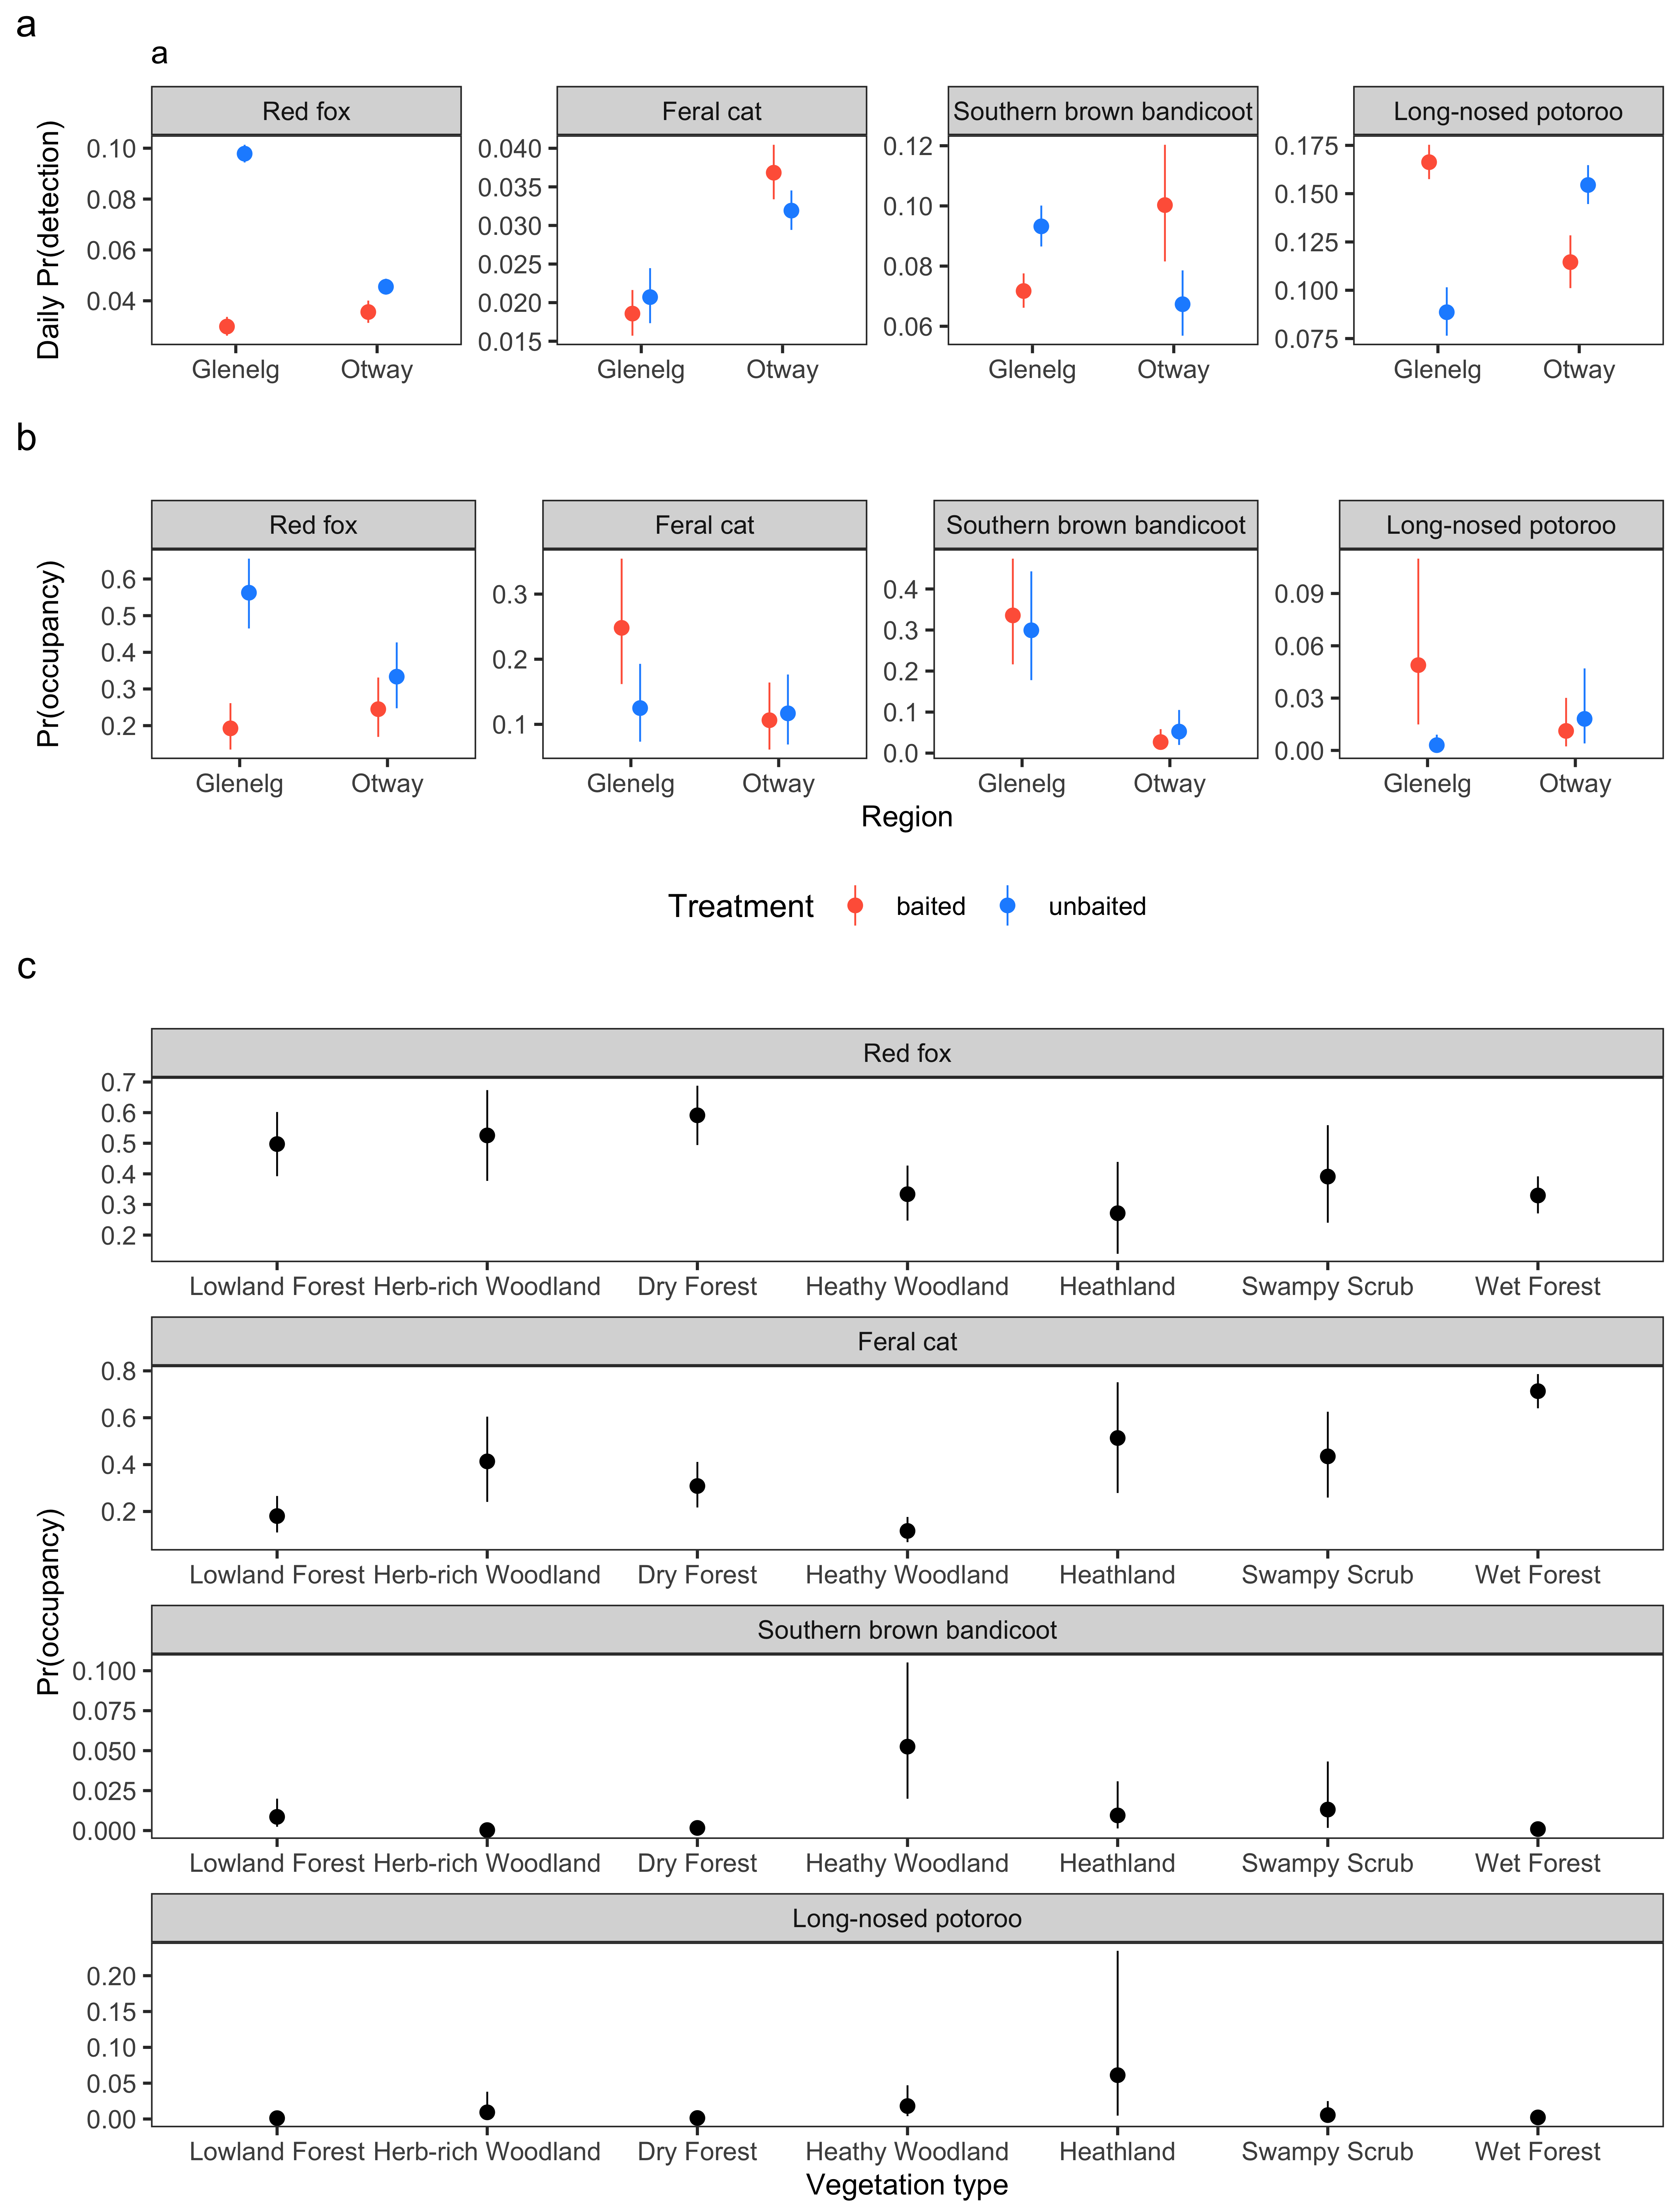
\includegraphics[width=0.8\linewidth]{../figs/occ_det_fox_control} 

}

\caption{Outputs from Bayesian occupancy-detection for each study species. Daily detection probabilities (a) and occupancy estimates (b) in landscapes with fox control (red) and without fox control (blue) in the Glenelg region and Otway Ranges, south-west Victoria, Australia (with Heathy Woodlands as a reference level). Fox control had occurred in The Glenelg region for 8 - 13 years and was monitored with a control-impact design. The Otway Ranges was monitored using a before-after-control-impact experimental design; surveyed approximately 1 year prior and 2 years following the commencement of fox-baiting. Occupancy was also modelled as a function of vegetation type (Ecological Vegetation Class groups; c). Error bars represent 95\% Bayesian credible intervals.}\label{fig:occ-det}
\end{figure}

\newpage

\begin{figure}

{\centering 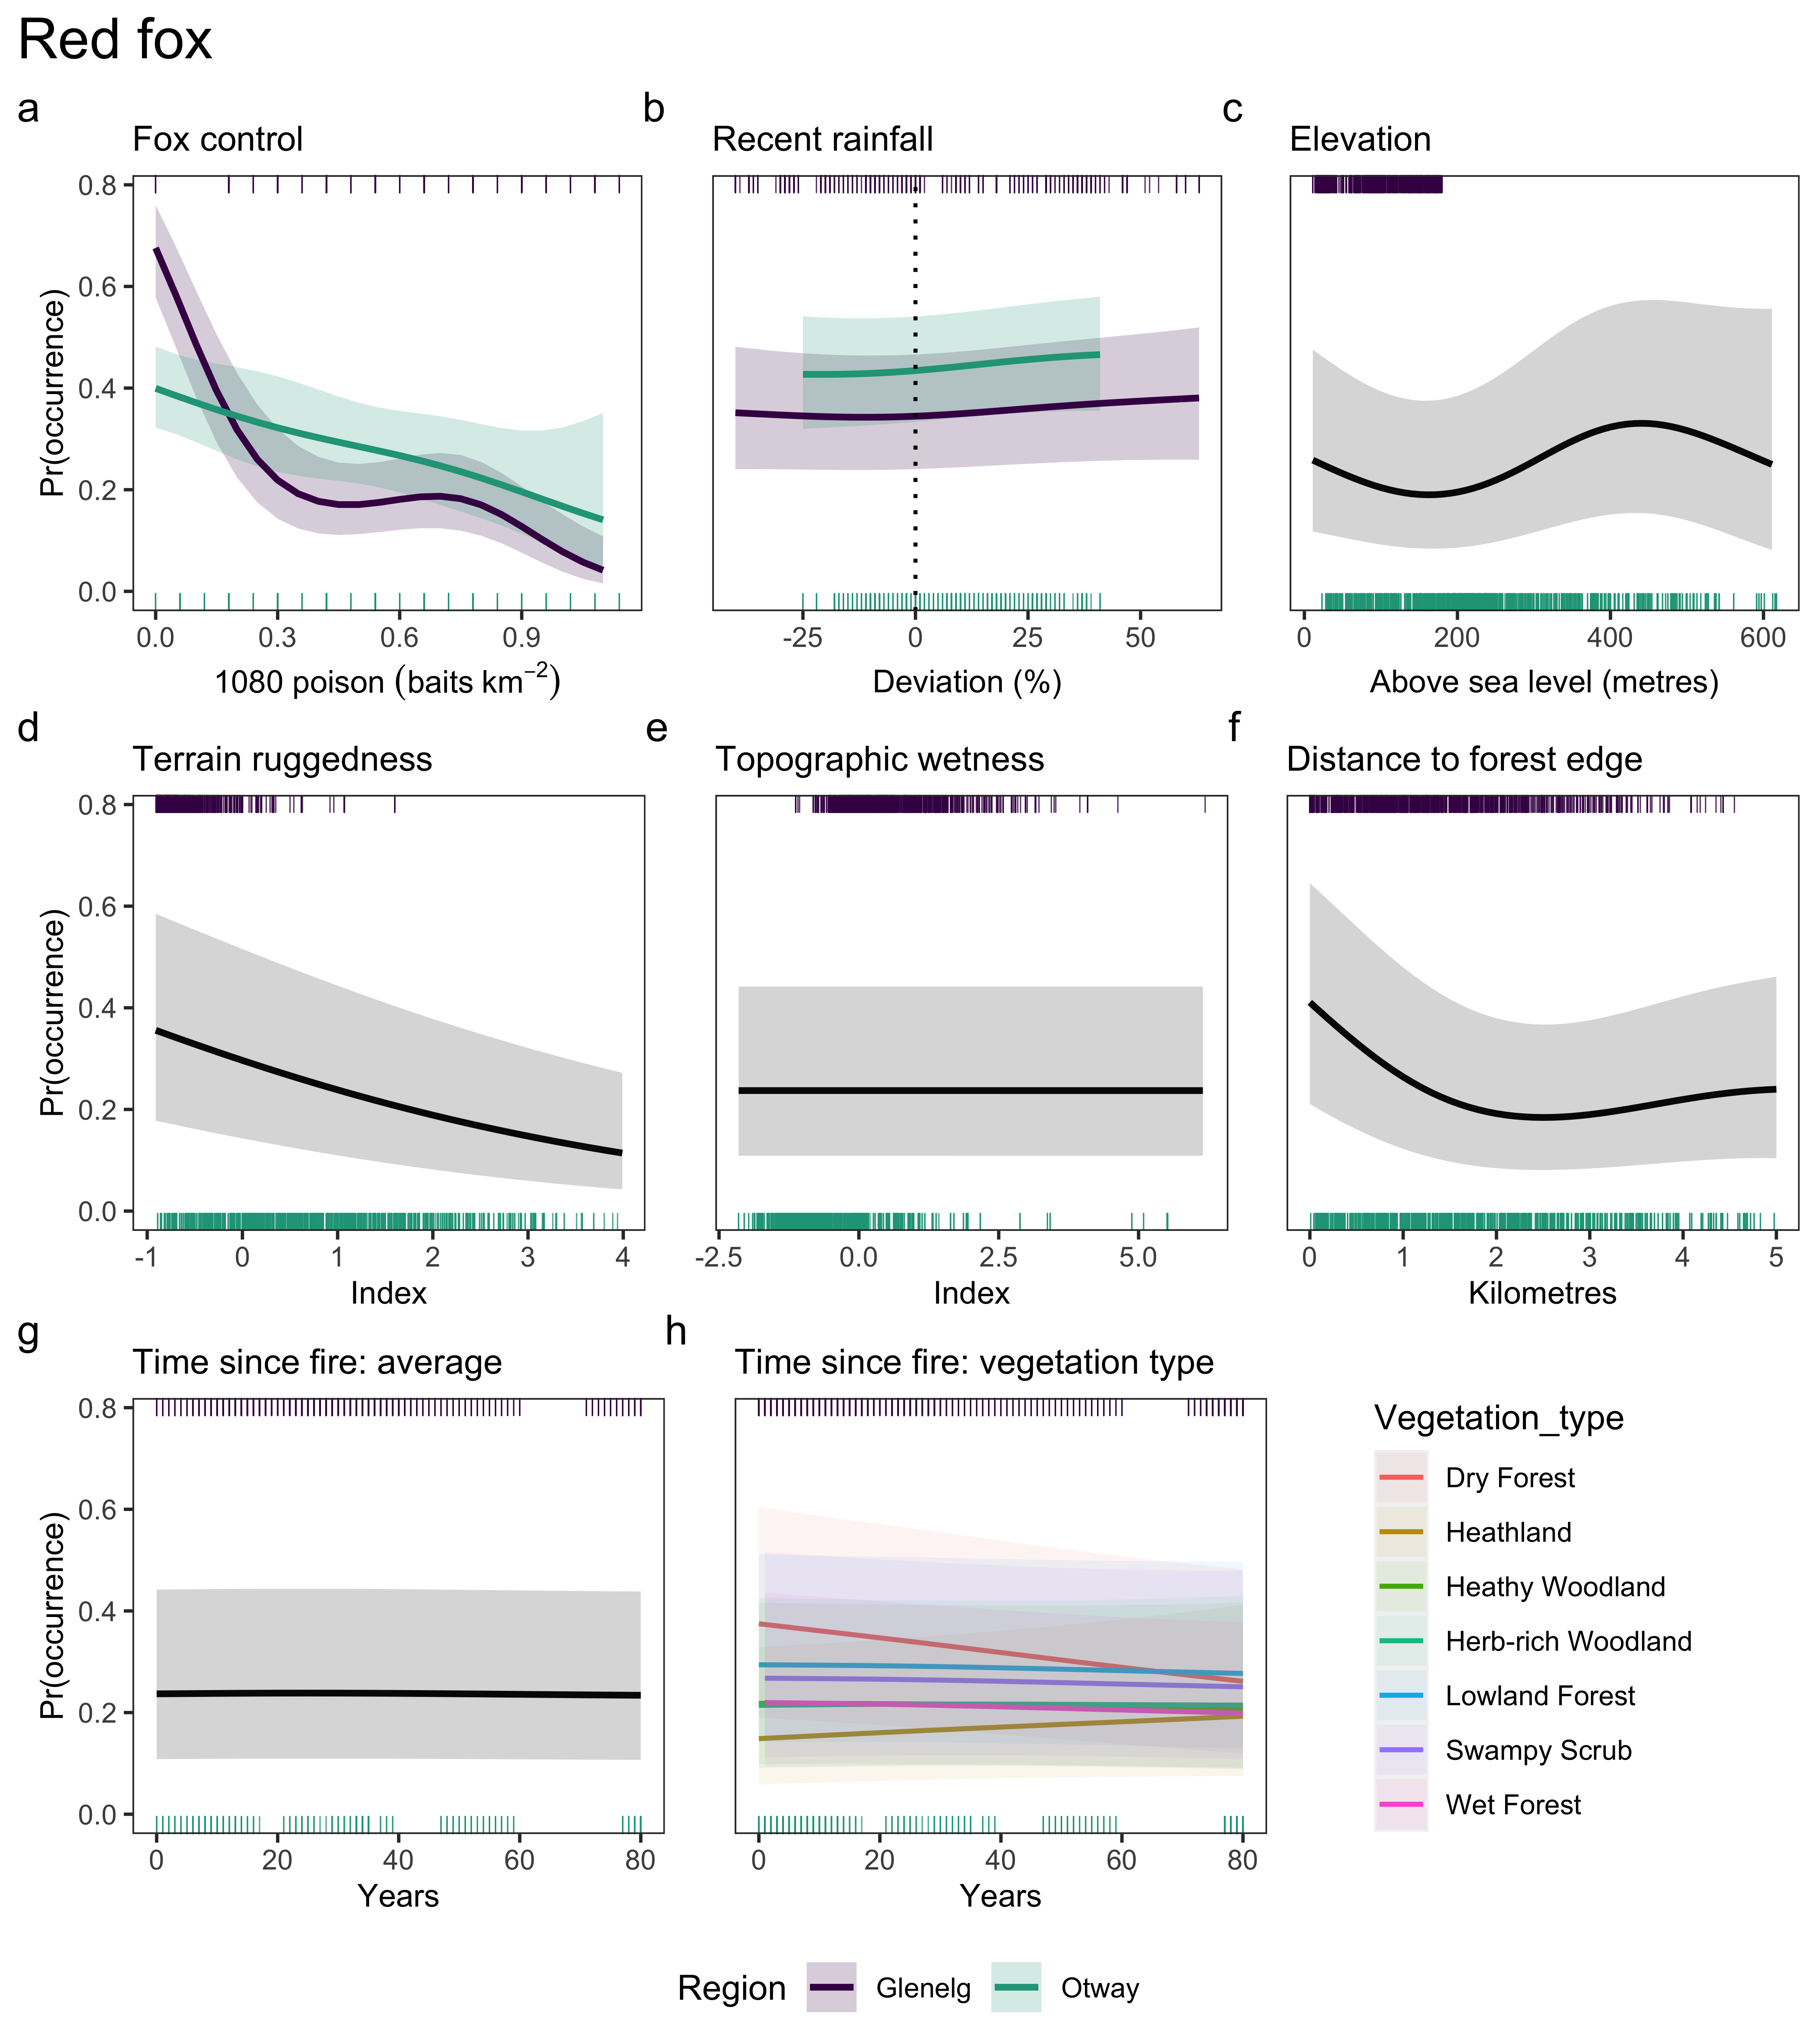
\includegraphics[width=0.8\linewidth]{../figs/gams_fox} 

}

\caption{Generalised additive model estimates of the effect of each explanatory variable (columns) on red fox \textit{Vulpes vulpes} occurrence. Shaded bands indicate 95\% confidence intervals.}\label{fig:gams-occ-fox}
\end{figure}

\newpage

\begin{figure}

{\centering 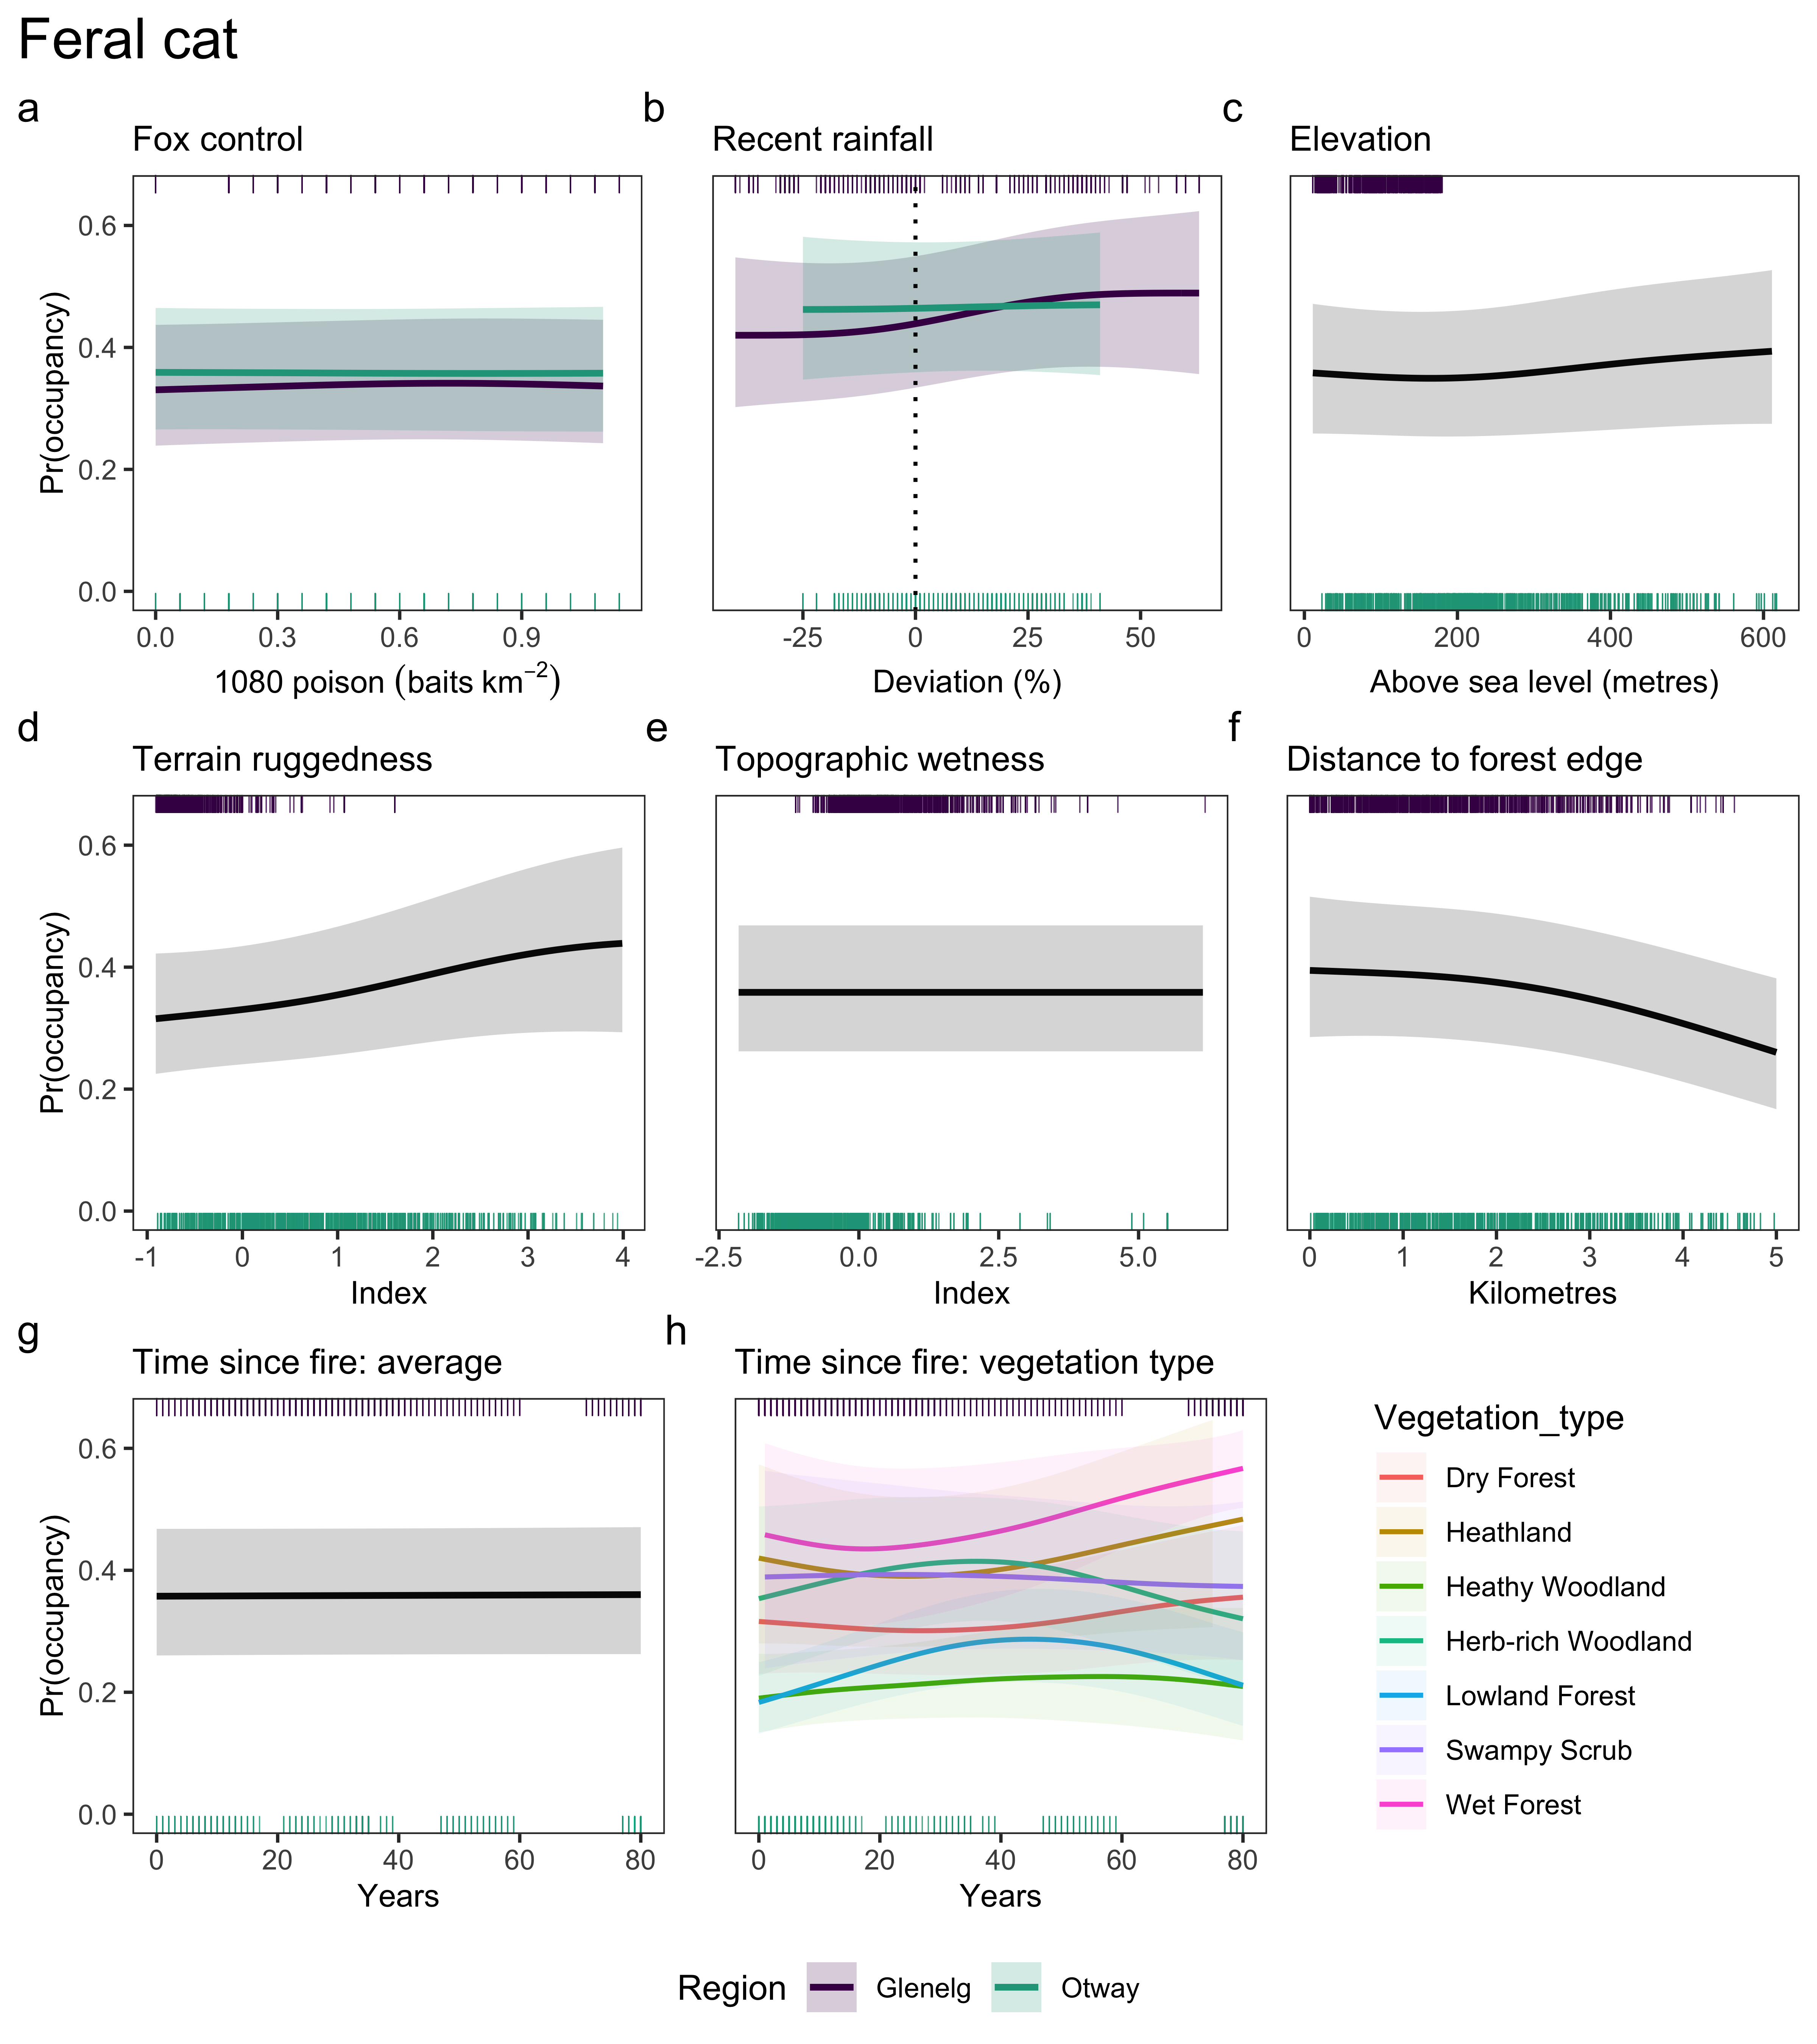
\includegraphics[width=0.8\linewidth]{../figs/gams_cat} 

}

\caption{Generalised additive model estimates of the effect of each explanatory variable (columns) on feral cat \textit{Felis catus} occurrence. Shaded bands indicate 95\% confidence intervals.}\label{fig:gams-occ-cat}
\end{figure}

\newpage

\begin{figure}

{\centering 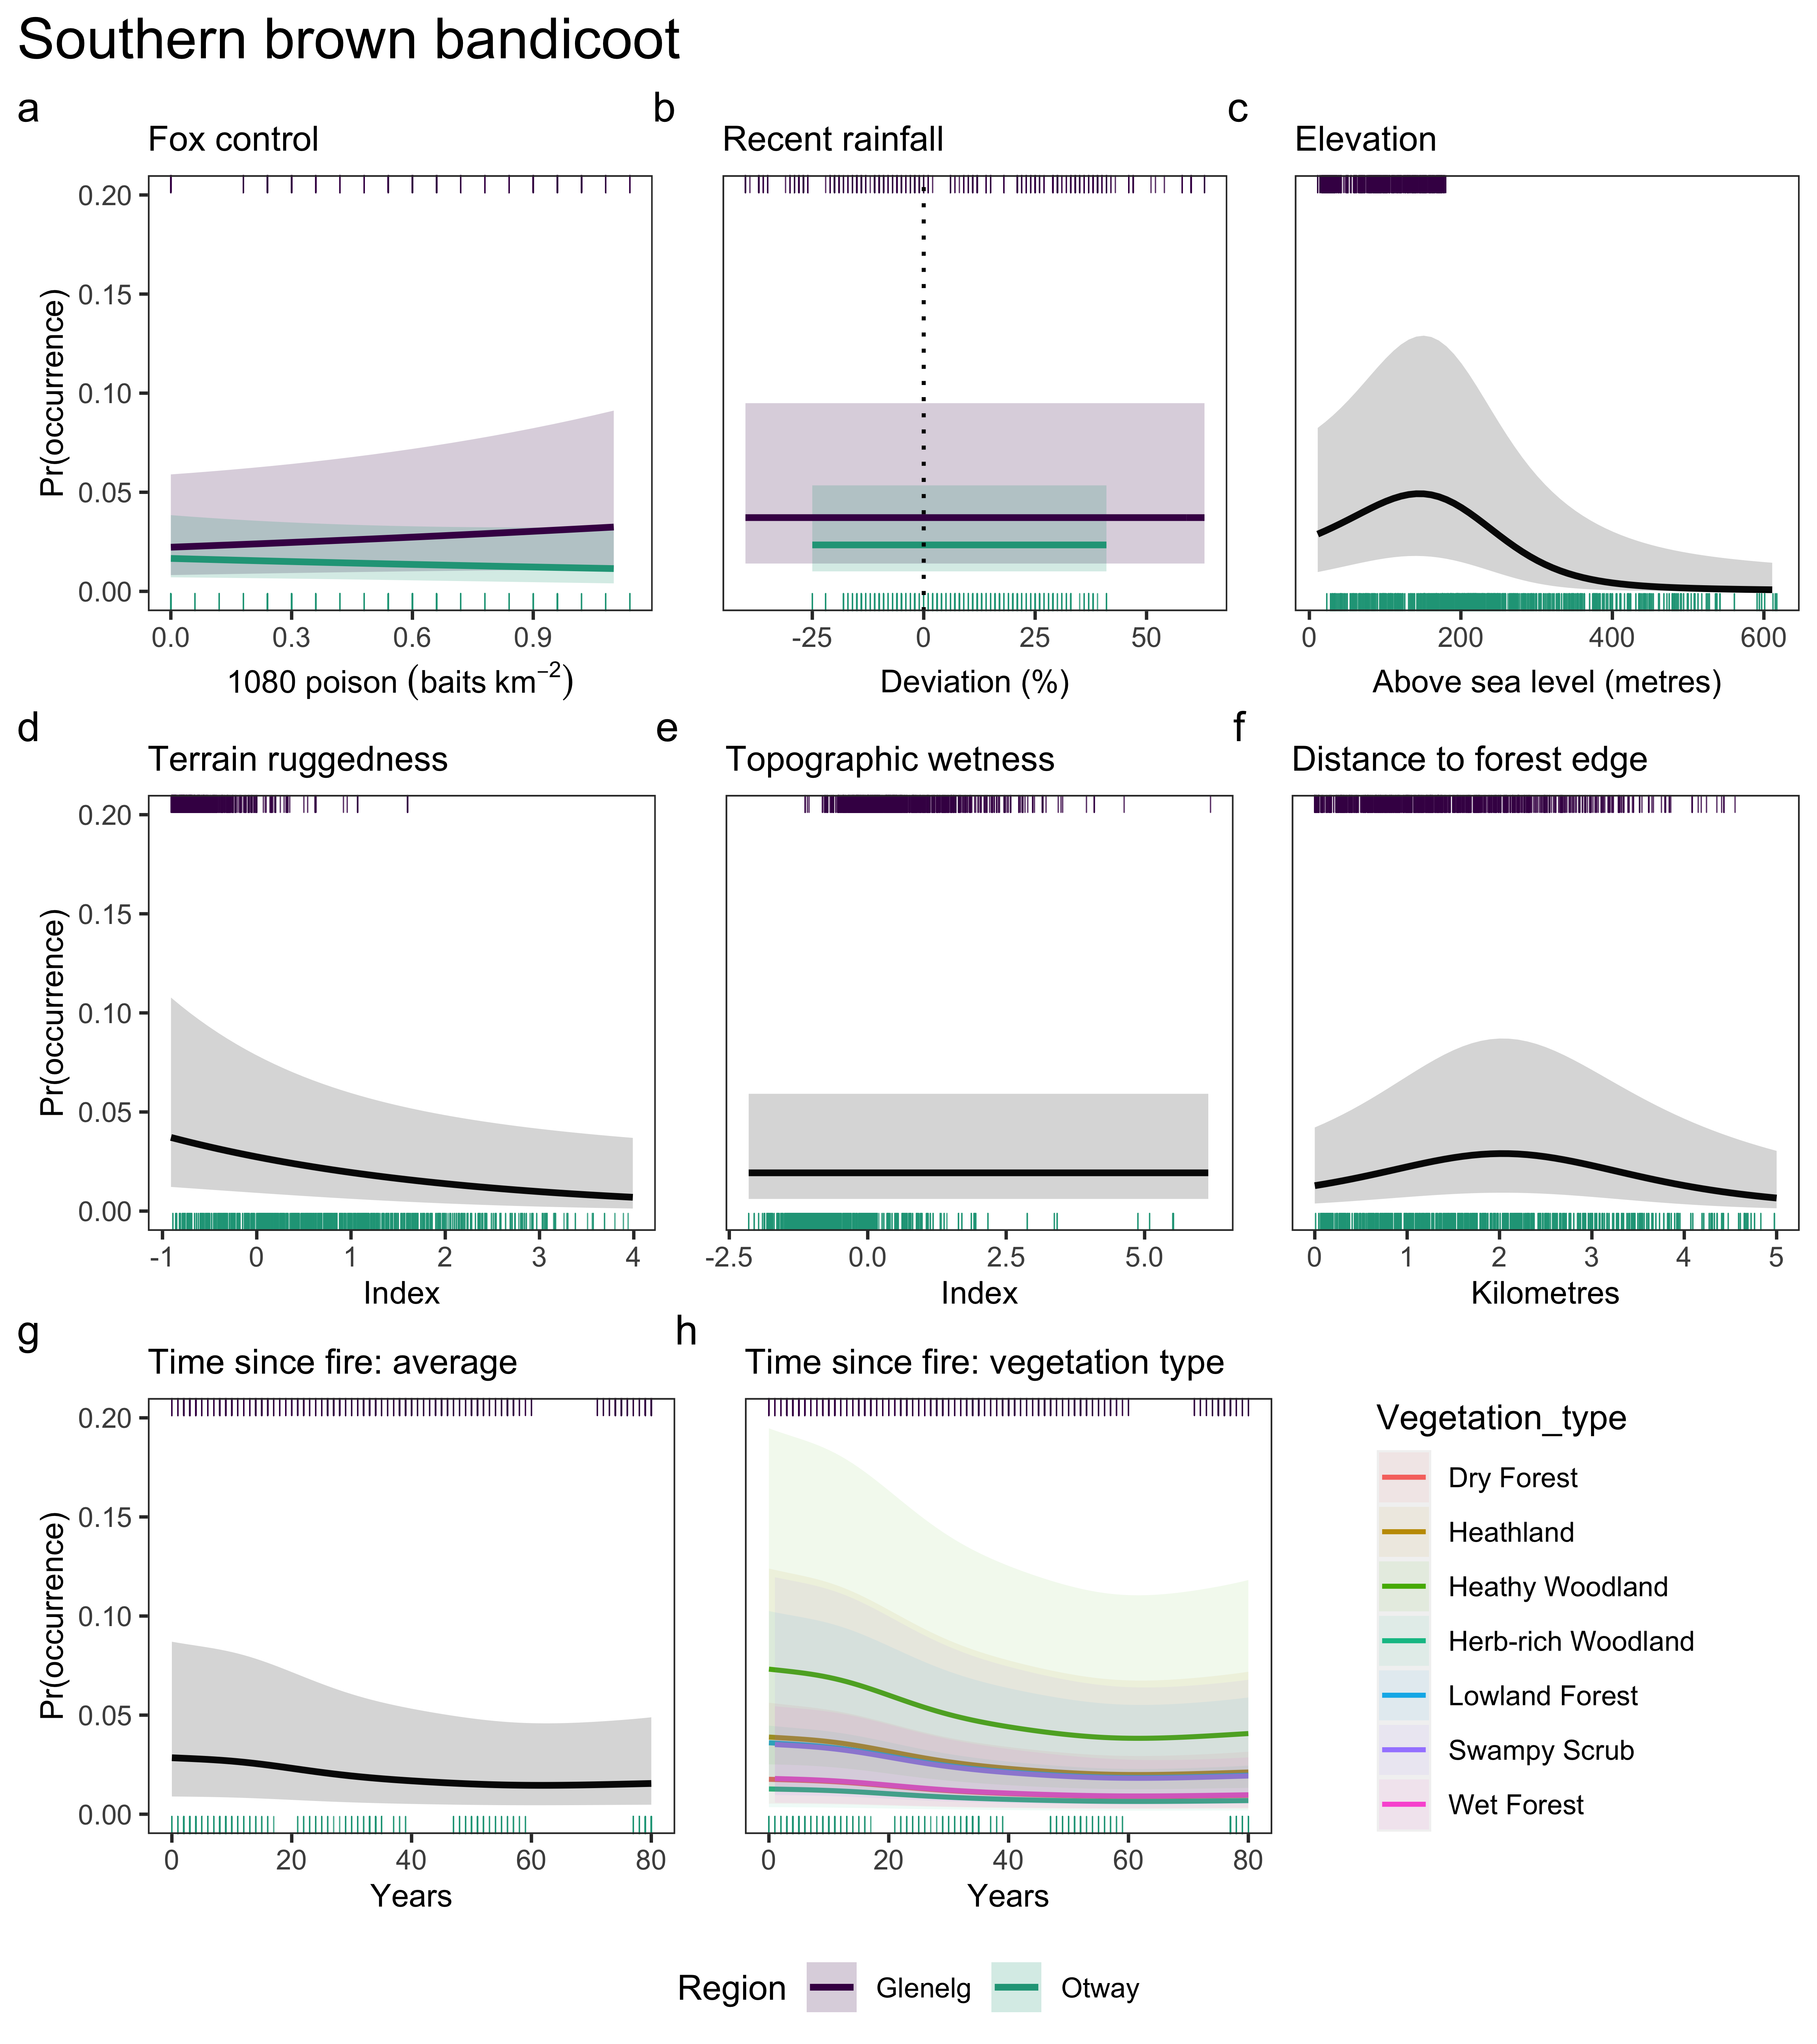
\includegraphics[width=0.8\linewidth]{../figs/gams_sbb} 

}

\caption{Generalised additive model estimates of the effect of each explanatory variable (columns) on southern brown bandicoot \textit{Isoodon obesulus} occurrence. Shaded bands indicate 95\% confidence intervals.}\label{fig:gams-occ-sbb}
\end{figure}

\newpage

\begin{figure}

{\centering 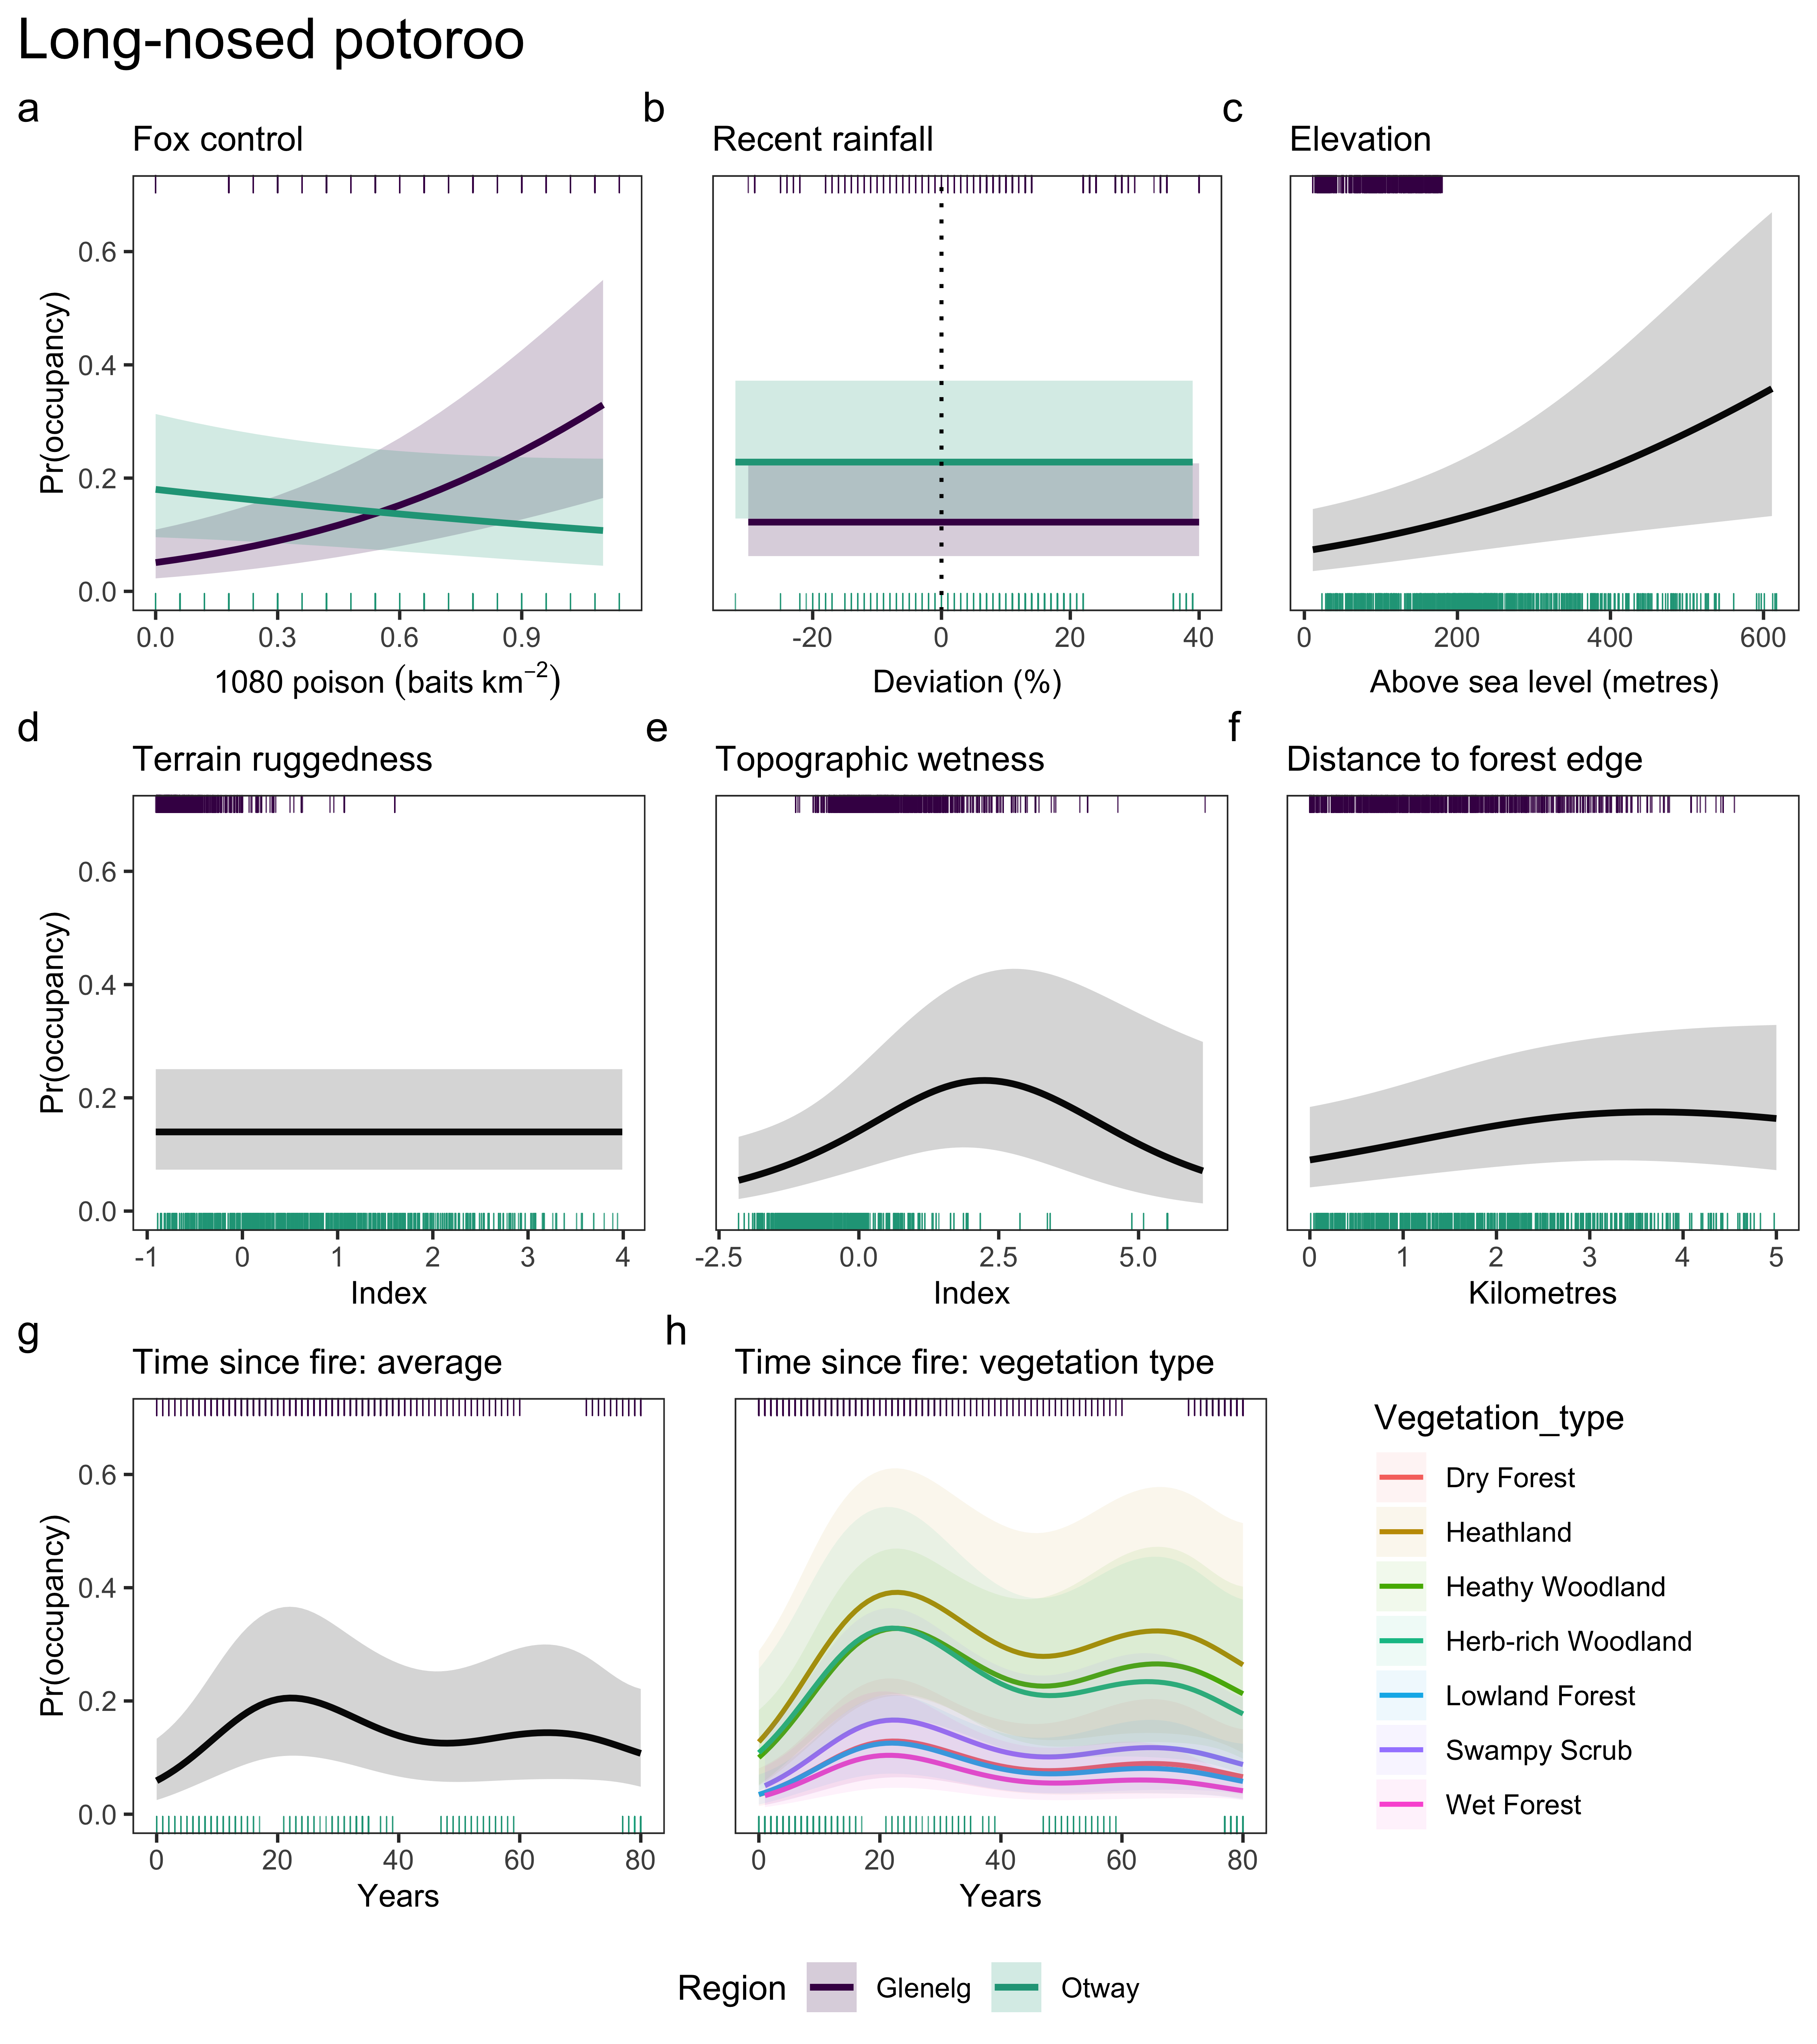
\includegraphics[width=0.8\linewidth]{../figs/gams_lnp} 

}

\caption{Generalised additive model estimates of the effect of each explanatory variable (columns) on long-nosed potoroo \textit{Potorous tridactylus} occurrence. Shaded bands indicate 95\% confidence intervals.}\label{fig:gams-occ-lnp}
\end{figure}

\newpage

\hypertarget{discussion}{%
\section{DISCUSSION}\label{discussion}}

Here we found that consistent and long-term lethal control can reduce a widespread invasive apex predator (fox) to a near-zero occurrence probability--and importantly--increase the occurrence probability of a threatened prey species (LNP) by more than 6-fold (Fig. \ref{fig:gams-occ-fox}a; Fig. \ref{fig:gams-occ-lnp}a). However, prey responses to predator suppression are not universal (Salo \emph{et al.} 2010; Hunter \emph{et al.} 2018; Duncan \emph{et al.} 2020). Despite signs of improvement in the early stages of the Glenelg Ark fox baiting program (Robley \emph{et al.} 2014), we found little evidence that SBB occupancy increased with fox control in either region (Fig. \ref{fig:occ-det}b; Fig. \ref{fig:gams-occ-lnp}a). This may have been because feral cat occupancy was twice as high in the landscapes with fox control relative to those without in the Glenelg region (Fig. \ref{fig:occ-det}b), potentially signalling mesopredator release. In the Otway region (where fox control recently commenced and baiting was less frequent), foxes were suppressed to a lesser extent and neither threatened prey species showed signs of improvement (Fig. \ref{fig:occ-det}b; Fig. \ref{fig:gams-occ-fox}a; Fig. \ref{fig:gams-occ-sbb}a; Fig. \ref{fig:gams-occ-lnp}a). Our study demonstrates that lethal invasive predator control can be a highly effective conservation strategy, but only for some species and when sustained continuously over the long-term.

The Glenelg Ark program has continuously controlled foxes across approximately 100 000 ha of public land since 2005 (Robley \emph{et al.} 2014) and is one of the few fox control programs in Australia to demonstrate a sustained reduction in fox occupancy (see also Stobo-Wilson \emph{et al.} 2020a). A reduction in fox occupancy is a strong sign of management effectiveness because it means prey are less exposed to the threat of predation. Our study provides empirical evidence that the effectiveness of fox control from poison-baiting programs depends on the density of poison-baits deployed (Fig. \ref{fig:gams-occ-fox}a). This has only previously been inferred by comparing fox baiting programs across different regions (where fox ecology, environmental conditions and study designs differ). The densities of poison-baits in our study regions (maximum 1.14 baits km\textsuperscript{-2}) were far below the recommended 5 - 10 baits km\textsuperscript{-2} (mostly derived from studies in arid and semi-arid regions; Saunders \& McLeod 2007), but nonetheless effective at fox suppression in the Glenelg region (Fig. \ref{fig:occ-det}b). Increasing bait density up to 0.3 baits km\textsuperscript{-2} was particularly effective at controlling foxes in the Glenelg region, reducing fox occurrence by up to four-fold compared to unbaited regions; afterwards, increasing poison-bait densities continued to suppress foxes, but with a weaker effect (Fig. \ref{fig:gams-occ-fox}a). Increased bait caching at high bait densities may explain why fox suppression tapered off, which is likely to result in a sublethal dose when eventually consumed and potential bait aversion (Saunders \& McLeod 2007). Nonetheless, benefits to threatened native prey is the best metric of fox control effectiveness. The probability of LNP occurrence increased linearly with poison-bait density in the Glenelg region (Fig. \ref{fig:gams-occ-lnp}a), confirming that high fox control effort leads to improved conservation outcomes.

We slightly underestimated the effect of bait density across both regions because the models assumed all bait-stations were constantly active, despite some bait-replacements being missed due to accessibility issues following wet weather events or because of more pressing management concerns (namely wildfire). We more strongly underestimated the effect of bait density in the Otway Ranges because we also did not account for a near six-month pause in bait replacement in 2018. We also expect fox-baits to be less effective in the Otway Ranges than the Glenelg region due to the higher rainfall which more quickly degrades the poison (Saunders, McLeod, \& Kay 2000; Gentle, Saunders, \& Dickman 2007). Nonetheless, fox occupancy in the Otway Ranges was still negatively associated with fox-bait density (Fig. \ref{fig:gams-occ-fox}a), suggesting that intensified and sustained fox control is likely to be effective in that region. Future research will benefit from accounting for the role of environmental conditions and prey availability on baiting effectiveness (Saunders \& McLeod 2007; Carter \& Luck 2013), as well as interference with baits by non-target species (Fairbridge \emph{et al.} 2000; Glen \& Dickman 2003; Marlow \emph{et al.} 2015).

Evidence that fox control caused mesopredator release of feral cats in terms of detectability and occupancy was mixed. Cat occupancy was higher in sites with fox control in the Glenelg region and cat detectability increased with fox control in the Otway Ranges (Fig. \ref{fig:occ-det}a:b). However, cat occurrence did not change across gradients of poison-bait density in either region (GAM; Fig. \ref{fig:gams-occ-cat}a). Cat detectability in the Glenelg region was very low (Fig. \ref{fig:occ-det}a), and so the model assumption of perfect detection in the cat GAM was likely problematic. This result could also signal that cats respond to fox suppression at the landscape level rather than at finer spatial scales. In addition, potential changes in population density and behaviour following mesopredator release (Brashares \emph{et al.} 2010), such as cats reducing their ranging behaviour following fox control (as found by Molsher \emph{et al.} 2017), could skew inference around occupancy estimates (Efford \& Dawson 2012; McCarthy \emph{et al.} 2013; Neilson \emph{et al.} 2018; Stewart \emph{et al.} 2018; Broadley \emph{et al.} 2019). Cats had weak associations with most explanatory variables, the poorest detection rates and worst model fits of our study species, further highlighting the challenges of monitoring this elusive, generalist predator (Fisher \emph{et al.} 2015; Stokeld \emph{et al.} 2015; Algar \emph{et al.} 2020).

In the Glenelg region, LNP--but not SBB--occupancy improved with fox control (Fig. \ref{fig:occ-det}b). Using increases in prey occupancy to measure the effectiveness of predator control rests on the assumption that there is suitable habitat for prey to expand into. While SBBs had a narrower distribution relative to LNPs across our study regions (largely absent from the wet forests), there were 34 heathy woodland sites in the Glenelg region where they were never observed (from 196 camera-trap deployments), suggesting there may have been suitable habitat for them to colonise. However, EVGs such as ``heathy woodland'' are a coarse, model-generated categories; there may have been an environmental variable which precluded SBB presence at these 34 sites, such as local habitat structure (Swan \emph{et al.} 2015), although Smith (2013) found no association between habitat structure and SBB occupancy in the 240 Glenelg Ark monitoring sites. Alternatively, the different prey responses in our study could reflect the relative vulnerability of these species to fox and cat predation: LNPs (and other small macropods) appear more strongly limited by fox predation, whereas SBBs tend to be more closely associated with cat populations (Arthur, Catling, \& Reid 2012; Hunter \emph{et al.} 2018) and so may have experienced negative consequences from higher cat occupancy in Glenelg landscapes with fox control. This would also help explain why SBB occupancy was highest in heathy woodlands, where cat occupancy was lowest (Fig. \ref{fig:occ-det}c). Formally testing whether invasive predator occupancy impacts the probability of prey occupancy using multispecies models (Rota \emph{et al.} 2016) is a priority for future research.

In the Otway Ranges, fox control did not improve SBB or LNP occupancy (Fig. \ref{fig:occ-det}b; Fig. \ref{fig:gams-occ-sbb}a); Fig. \ref{fig:gams-occ-lnp}a). This is unsurprising given fox suppression in the Otway Ranges was weak, likely because fox control had only recently commenced and bait replacement was relatively inconsistent. Despite the high fecundity of these prey species, two years was may have been insufficient time to measure an effect of fox control on prey occupancy. Additionally, we averaged fox control effects over a 0 - 2 year post-baiting time period in the Otway Ranges; although, our findings concur with those of Robley, Moloney, \& Parks Victoria West Coast District Team (2019), who estimated annual occupancy probabilities using a more traditional BACI analysis with a subset of this data. The ongoing broadscale monitoring of the Otway Ark fox control program and other local initiatives will shed light on occupancy trends over time.

Fire can have long-term impacts on the occurrence of small-medium sized native mammals (Claridge \& Barry 2000; Monamy \& Fox 2000; Arthur, Catling, \& Reid 2012). Previously, Smith (2013) found extinction probabilities for both LNPs and SBBs to be high for up to 18 months post-fire. Here we found that, LNP occurrence was low immediately post-fire and peaked 20 years post-fire (Fig. \ref{fig:gams-occ-lnp}g). However, seemingly contrary to Smith (2013), SBB occurrence declined with increasing TSF (Fig. \ref{fig:gams-occ-sbb}g). Given the uncertainty around our estimates and importance for managers implementing prescribed fire, further research is required to clarify and understand the mechanisms behind these responses to fire. A key remaining question is whether fox control impacts these species' responses to fire in the short and long-term.

While there is now considerable research which has demonstrated that invasive predator impacts are heightened in recently burnt areas (Meek \& Saunders 2000; Green \& Sanecki 2006; McGregor \emph{et al.} 2014, 2016; Leahy \emph{et al.} 2016; Hradsky \emph{et al.} 2017b; a), we have a comparatively poor understanding of how long-term fire patterns impact invasive predators (reviewed in Hradsky 2020). Similar to many previous studies, we found no average response to TSF for foxes or cats, however, both predators had varying responses to TSF across vegetation types (Fig. \ref{fig:gams-occ-fox}g:h; Fig. \ref{fig:gams-occ-cat}g:h;). This supports the `dynamic vegetation' hypothesis (Nimmo \emph{et al.} 2014); the first evidence of this kind for predators (albiet uncertainty around these relationships was high). Studies often merge similar vegetation types due to some groups having small sample sizes, however, we found no clear way of grouping vegetation types that was relevant to multiple species. Our hierarchical specification of the TSF and vegetation type interaction was powerful in this regard as it allowed separate responses for each vegetation type, while sharing information across vegetation types, and provided confidence that there was data to back-up differently shaped responses given the penalisation to the average response (Pedersen \emph{et al.} 2019).

Accounting for other drivers of species in models that estimate responses to management is critical, but not often undertaken. For example, unexpected declines and local extinctions of small-medium sized mammals have occurred following 40 years of fox control in south-west Western Australia are posited to be the result of a mesopredator release of cats; Wayne \emph{et al.} (2017){]}, but the Intergovernmental Panel on Climate Change has identified this region as a `drying hotspot' (Kala \emph{et al.} 2021) and there also are strong concerns around the intensity of prescribed fire operations (e.g., Bennett \& Edwards 2021), offering alternative or contributing explanations for prey declines. Mammal communities have also collapsed following long-term fox-control in Booderee National Park (Lindenmayer \emph{et al.} 2018), but a severe wildlife burnt through approximately half the region in the same year fox control commenced (leaving greater than 73\% of park burnt within the last decade; Foster \emph{et al.} 2017). Similarly, recent fire events have been skewed towards the baited landscapes of the Glenelg region since fox control began, with the majority of long-unburnt vegetation occurring in unbaited landscapes (Fig. \ref{fig:veg-tsf-violin}). We were partially able to compensate for this confounding by including an additional 424 sites in the Glenelg region, as well as the Otway Ranges datasets--providing a wider range of fire history patterns in each vegetation type with and without fox control (Fig. \ref{fig:veg-tsf-violin}). Our study demonstrates the value of bringing together multiple smaller datasets to compare management effectiveness.

Occurrence models are powerful tools to predict species distributions but less useful for explaining fine-scale site-use for wide-ranging, generalist species in continuous habitat (Efford \& Dawson 2012; Guillera-Arroita \emph{et al.} 2015). Despite our large dataset, uncertainty for most explanatory variables was high and their inclusion offered little improvement to GAM fits relative to null models (in fact, slightly worsened the model fit for foxes; Table. \ref{tab:occ-model-sumstats}). Our study offers little additional clarity about the `natural' drivers of occurrence for invasive predators and medium-sized mammalian prey within their distributions other than clarifying the importance of broad vegetation type. While we did seek to provide inference on what drives the patchy distributions of these species, our key aim was to account for confounding variables while testing fox control effects. Nevertheless, testing the predictive performance of distribution models for these species with independent datasets, in particular whether region-specific or across-region models predict more accurately, will aid the management of these species.

Fox control is a major expenditure of Australian conservation and agricultural programs (approximately AUD 16 million annually; McLeod \& Norris 2004). It is critical to ensure cost-effectiveness from both a monetary and ethical standpoint. Here we demonstrate clearly that effectiveness in terms of fox suppression is a function of control effort. However, the evidence for benefits to native prey species was mixed. Prey may not benefit from predator control if it leads to mesopredator release of other invasive predators, or if prey are constrained by other factors such as lack of suitable habitat. Species vulnerable to fox predation are also sensitive to fire-induced changes in habitat structure (Woinarski, Burbidge, \& Harrison 2015), and so integrating conservation strategies that consider habitat and invasive predator management in concert is a future priority. Our work highlights the importance of fine-scale monitoring, considering multiple drivers and tailoring conservation strategies to local contexts.

\newpage

\hypertarget{acknowledgements}{%
\section*{ACKNOWLEDGEMENTS}\label{acknowledgements}}
\addcontentsline{toc}{section}{ACKNOWLEDGEMENTS}

\newpage

\hypertarget{references}{%
\section*{REFERENCES}\label{references}}
\addcontentsline{toc}{section}{REFERENCES}

\hypertarget{refs}{}
\leavevmode\hypertarget{ref-algar2020feral}{}%
Algar, D., Johnston, M., Tiller, C., Onus, M., Fletcher, J., Desmond, G., Hamilton, N. \& Speldewinde, P. (2020) Feral cat eradication on Dirk Hartog Island, Western Australia. \emph{Biological Invasions}, \textbf{22}, 1037--1054.

\leavevmode\hypertarget{ref-arthur2012relative}{}%
Arthur, A.D., Catling, P.C. \& Reid, A. (2012) Relative influence of habitat structure, species interactions and rainfall on the post-fire population dynamics of ground-dwelling vertebrates. \emph{Austral Ecology}, \textbf{37}, 958--970.

\leavevmode\hypertarget{ref-ballari2016potential}{}%
Ballari, S.A., Kuebbing, S.E. \& Nuñez, M.A. (2016) Potential problems of removing one invasive species at a time: A meta-analysis of the interactions between invasive vertebrates and unexpected effects of removal programs. \emph{PeerJ}, \textbf{4}, e2029.

\leavevmode\hypertarget{ref-banks1999predation}{}%
Banks, P.B. (1999) Predation by introduced foxes on native bush rats in Australia: Do foxes take the doomed surplus? \emph{Journal of Applied Ecology}, \textbf{36}, 1063--1071.

\leavevmode\hypertarget{ref-baxter2008cost}{}%
Baxter, P.W., Sabo, J.L., Wilcox, C., McCarthy, M.A. \& Possingham, H.P. (2008) Cost-effective suppression and eradication of invasive predators. \emph{Conservation Biology}, \textbf{22}, 89--98.

\leavevmode\hypertarget{ref-bellard2016global}{}%
Bellard, C., Genovesi, P. \& Jeschke, J. (2016) Global patterns in threats to vertebrates by biological invasions. \emph{Proceedings of the Royal Society B: Biological Sciences}, \textbf{283}, 20152454.

\leavevmode\hypertarget{ref-bennett2021prescribed}{}%
Bennett, M. \& Edwards, T. (2021) Prescribed burn devastates one of WA's last two endangered numbat habitats, \url{https://www.abc.net.au/news/2021-05-02/prescribed-burn-decimates-numbat-habitat-wa/100110960}

\leavevmode\hypertarget{ref-benshemesh2020citizen}{}%
Benshemesh, J., Southwell, D., Barker, R. \& McCarthy, M. (2020) Citizen scientists reveal nationwide trends and drivers in the breeding activity of a threatened bird, the malleefowl \emph{(Leipoa ocellata)}. \emph{Biological Conservation}, \textbf{246}, 108573.

\leavevmode\hypertarget{ref-beven1979physically}{}%
Beven, K.J. \& Kirkby, M.J. (1979) A physically based, variable contributing area model of basin hydrology. \emph{Hydrological Sciences Journal}, \textbf{24}, 43--69.

\leavevmode\hypertarget{ref-brashares2010ecological}{}%
Brashares, J.S., Prugh, L.R., Stoner, C.J. \& Epps, C.W. (2010) Ecological and conservation implications of mesopredator release. \emph{Trophic cascades: predators, prey, and the changing dynamics of nature}, 221--240.

\leavevmode\hypertarget{ref-braysher2017managing}{}%
Braysher, M. (2017) \emph{Managing Australia's Pest Animals: A Guide to Strategic Planning and Effective Management}. CSIRO Publishing.

\leavevmode\hypertarget{ref-broadley2019density}{}%
Broadley, K., Burton, A.C., Avgar, T. \& Boutin, S. (2019) Density-dependent space use affects interpretation of camera trap detection rates. \emph{Ecology and Evolution}, \textbf{9}, 14031--14041.

\leavevmode\hypertarget{ref-BOM2021}{}%
Bureau of Meteorology. (2021) Climate data online.

\leavevmode\hypertarget{ref-burnham2004multimodel}{}%
Burnham, K.P. \& Anderson, D.R. (2004) Multimodel inference: Understanding AIC and BIC in model selection. \emph{Sociological Methods \& Research}, \textbf{33}, 261--304.

\leavevmode\hypertarget{ref-carpenter2017stan}{}%
Carpenter, B., Gelman, A., Hoffman, M.D., Lee, D., Goodrich, B., Betancourt, M., Brubaker, M., Guo, J., Li, P. \& Riddell, A. (2017) Stan: A probabilistic programming language. \emph{Journal of Statistical Software}, \textbf{76}, 1--32.

\leavevmode\hypertarget{ref-carter2013fox}{}%
Carter, A. \& Luck, G.W. (2013) Fox baiting in agricultural landscapes: Preliminary findings on the importance of bait-site selection. \emph{Wildlife Research}, \textbf{40}, 184--195.

\leavevmode\hypertarget{ref-cattarino2016accounting}{}%
Cattarino, L., Hermoso, V., Bradford, L.W., Carwardine, J., Wilson, K.A., Kennard, M.J. \& Linke, S. (2016) Accounting for continuous species' responses to management effort enhances cost-effectiveness of conservation decisions. \emph{Biological Conservation}, \textbf{197}, 116--123.

\leavevmode\hypertarget{ref-christie2020poor}{}%
Christie, A.P., Amano, T., Martin, P.A., Petrovan, S.O., Shackelford, G.E., Simmons, B.I., Smith, R.K., Williams, D.R., Wordley, C.F. \& Sutherland, W.J. (2020) Poor availability of context-specific evidence hampers decision-making in conservation. \emph{Biological Conservation}, \textbf{248}, 108666.

\leavevmode\hypertarget{ref-claridge2000factors}{}%
Claridge, A.W. \& Barry, S.C. (2000) Factors influencing the distribution of medium-sized ground-dwelling mammals in southeastern mainland Australia. \emph{Austral Ecology}, \textbf{25}, 676--688.

\leavevmode\hypertarget{ref-clarke2008catering}{}%
Clarke, M.F. (2008) Catering for the needs of fauna in fire management: Science or just wishful thinking? \emph{Wildlife Research}, \textbf{35}, 385--394.

\leavevmode\hypertarget{ref-collins2012can}{}%
Collins, L., Bradstock, R.A., Tasker, E.M. \& Whelan, R.J. (2012) Can gullies preserve complex forest structure in frequently burnt landscapes? \emph{Biological Conservation}, \textbf{153}, 177--186.

\leavevmode\hypertarget{ref-courchamp1999cats}{}%
Courchamp, F., Langlais, M. \& Sugihara, G. (1999) Cats protecting birds: Modelling the mesopredator release effect. \emph{Journal of Animal Ecology}, \textbf{68}, 282--292.

\leavevmode\hypertarget{ref-crooks1999mesopredator}{}%
Crooks, K.R. \& Soulé, M.E. (1999) Mesopredator release and avifaunal extinctions in a fragmented system. \emph{Nature}, \textbf{400}, 563--566.

\leavevmode\hypertarget{ref-NV2005_EVCBCS}{}%
Department of Environment, Land, Water \& Planning. (2019) Native vegetation - modelled 2005 ecological vegetation classes (with bioregional conservation status), \url{http://services.land.vic.gov.au/catalogue/metadata?anzlicId=ANZVI0803003495\&publicId=guest\&extractionProviderId=1}

\leavevmode\hypertarget{ref-delwp2020bioregions}{}%
Department of Environment, Land, Water \& Planning. (2020a) Bioregions and EVC Benchmarks, \url{https://www.environment.vic.gov.au/biodiversity/bioregions-and-evc-benchmarks}

\leavevmode\hypertarget{ref-delwp2020elevation}{}%
Department of Environment, Land, Water \& Planning. (2020b) Vicmap elevation DEM 10m, \url{https://www.land.vic.gov.au/maps-and-spatial/spatial-data/vicmap-catalogue/vicmap-elevation}

\leavevmode\hypertarget{ref-doherty2015multiple}{}%
Doherty, T.S., Dickman, C.R., Nimmo, D.G. \& Ritchie, E.G. (2015) Multiple threats, or multiplying the threats? Interactions between invasive predators and other ecological disturbances. \emph{Biological Conservation}, \textbf{190}, 60--68.

\leavevmode\hypertarget{ref-doherty2016invasive}{}%
Doherty, T.S., Glen, A.S., Nimmo, D.G., Ritchie, E.G. \& Dickman, C.R. (2016) Invasive predators and global biodiversity loss. \emph{Proceedings of the National Academy of Sciences}, \textbf{113}, 11261--11265.

\leavevmode\hypertarget{ref-duncan2020eruptive}{}%
Duncan, R.P., Dexter, N., Wayne, A. \& Hone, J. (2020) Eruptive dynamics are common in managed mammal populations. \emph{Ecology}, \textbf{101}, e03175.

\leavevmode\hypertarget{ref-efford2012occupancy}{}%
Efford, M.G. \& Dawson, D.K. (2012) Occupancy in continuous habitat. \emph{Ecosphere}, \textbf{3}, 1--15.

\leavevmode\hypertarget{ref-evans2011spatial}{}%
Evans, M.C., Watson, J.E., Fuller, R.A., Venter, O., Bennett, S.C., Marsack, P.R. \& Possingham, H.P. (2011) The spatial distribution of threats to species in Australia. \emph{Bioscience}, \textbf{61}, 281--289.

\leavevmode\hypertarget{ref-fairbridge2000observations}{}%
Fairbridge, D., Fisher, P., Busana, F., Pontin, K. \& Edwards, A. (2000) Observations of the behaviour of free living bush rat, \emph{Rattus fuscipes} and southern brown bandicoot, \emph{Isoodon obesulus} at buried bait stations. \emph{Australian Mammalogy}, \textbf{22}, 125--127.

\leavevmode\hypertarget{ref-fisher2015cat}{}%
Fisher, P., Algar, D., Murphy, E., Johnston, M. \& Eason, C. (2015) How does cat behaviour influence the development and implementation of monitoring techniques and lethal control methods for feral cats? \emph{Applied Animal Behaviour Science}, \textbf{173}, 88--96.

\leavevmode\hypertarget{ref-fleming1996ground}{}%
Fleming, P.J. (1996) Ground-placed baits for the control of wild dogs: evaluation of a replacement-baiting strategy in north-eastern New South Wales. \emph{Wildlife Research}, \textbf{23}, 729--740.

\leavevmode\hypertarget{ref-foster2017effects}{}%
Foster, C., Barton, P., Robinson, N., MacGregor, C. \& Lindenmayer, D.B. (2017) Effects of a large wildfire on vegetation structure in a variable fire mosaic. \emph{Ecological applications}, \textbf{27}, 2369--2381.

\leavevmode\hypertarget{ref-gallant2012topographic}{}%
Gallant, J. \& Austin, J. (2012) Topographic Wetness Index derived from 1'' SRTM DEM-H. V2. 11 CSIRO. Data Collection.

\leavevmode\hypertarget{ref-garrard2008when}{}%
Garrard, G.E., Bekkessy, S.A., McCarthy, M.A. \& Wintle, B.A. (2008) When have we looked hard enough? A novel method for setting minimum survey effort protocols for flora surveys. \emph{Austral Ecology}, \textbf{33}, 986--998.

\leavevmode\hypertarget{ref-geary2020predators}{}%
Geary, W.L., Hradsky, B.A., Robley, A. \& Wintle, B.A. (2020) Predators, fire or resources: What drives the distribution of herbivores in fragmented mesic forests? \emph{Austral Ecology}, \textbf{45}, 329--339.

\leavevmode\hypertarget{ref-gentle2007persistence}{}%
Gentle, M., Saunders, G. \& Dickman, C. (2007) Persistence of sodium monofluoroacetate (1080) in fox baits and implications for fox management in south-eastern Australia. \emph{Wildlife Research}, \textbf{34}, 325--333.

\leavevmode\hypertarget{ref-glen2003monitoring}{}%
Glen, A.S. \& Dickman, C.R. (2003) Monitoring bait removal in vertebrate pest control: A comparison using track identification and remote photography. \emph{Wildlife Research}, \textbf{30}, 29--33.

\leavevmode\hypertarget{ref-glen2005complex}{}%
Glen, A.S. \& Dickman, C.R. (2005) Complex interactions among mammalian carnivores in Australia, and their implications for wildlife management. \emph{Biological Reviews}, \textbf{80}, 387--401.

\leavevmode\hypertarget{ref-green2006immediate}{}%
Green, K. \& Sanecki, G. (2006) Immediate and short-term responses of bird and mammal assemblages to a subalpine wildfire in the snowy mountains, Australia. \emph{Austral Ecology}, \textbf{31}, 673--681.

\leavevmode\hypertarget{ref-greenville2014bottom}{}%
Greenville, A.C., Wardle, G.M., Tamayo, B. \& Dickman, C.R. (2014) Bottom-up and top-down processes interact to modify intraguild interactions in resource-pulse environments. \emph{Oecologia}, \textbf{175}, 1349--1358.

\leavevmode\hypertarget{ref-guillera2015my}{}%
Guillera-Arroita, G., Lahoz-Monfort, J.J., Elith, J., Gordon, A., Kujala, H., Lentini, P.E., McCarthy, M.A., Tingley, R. \& Wintle, B.A. (2015) Is my species distribution model fit for purpose? Matching data and models to applications. \emph{Global Ecology and Biogeography}, \textbf{24}, 276--292.

\leavevmode\hypertarget{ref-hale2016fire}{}%
Hale, S., Nimmo, D.G., Cooke, R., Holland, G., James, S., Stevens, M., De Bondi, N., Woods, R., Castle, M., Campbell, K., Senior, K., Cassidy, S., Duffy, R., Holmes, B. \& White, J.G. (2016) Fire and climatic extremes shape mammal distributions in a fire-prone landscape. \emph{Diversity and Distributions}, \textbf{22}, 1127--1138.

\leavevmode\hypertarget{ref-haslem2011habitat}{}%
Haslem, A., Kelly, L.T., Nimmo, D.G., Watson, S.J., Kenny, S.A., Taylor, R.S., Avitabile, S.C., Callister, K.E., Spence-Bailey, L.M., Clarke, M.F. \& Bennett, A.F. (2011) Habitat or fuel? Implications of long-term, post-fire dynamics for the development of key resources for fauna and fire. \emph{Journal of Applied Ecology}, \textbf{48}, 247--256.

\leavevmode\hypertarget{ref-hohnen2016occupancy}{}%
Hohnen, R., Tuft, K., McGregor, H.W., Legge, S., Radford, I.J. \& Johnson, C.N. (2016) Occupancy of the invasive feral cat varies with habitat complexity. \emph{PLoS One}, \textbf{11}, e0152520.

\leavevmode\hypertarget{ref-hradsky2020conserving}{}%
Hradsky, B.A. (2020) Conserving Australia's threatened native mammals in predator-invaded, fire-prone landscapes. \emph{Wildlife Research}, \textbf{47}, 1--15.

\leavevmode\hypertarget{ref-hradsky2017responses}{}%
Hradsky, B.A., Mildwaters, C., Ritchie, E.G., Christie, F. \& Di Stefano, J. (2017a) Responses of invasive predators and native prey to a prescribed forest fire. \emph{Journal of Mammalogy}, \textbf{98}, 835--847.

\leavevmode\hypertarget{ref-hradsky2017human}{}%
Hradsky, B.A., Robley, A., Alexander, R., Ritchie, E.G., York, A. \& Di Stefano, J. (2017b) Human-modified habitats facilitate forest-dwelling populations of an invasive predator, \emph{(Vulpes vulpes)}. \emph{Scientific Reports}, \textbf{7}, 1--12.

\leavevmode\hypertarget{ref-hunter2018not}{}%
Hunter, D.O., Lagisz, M., Leo, V., Nakagawa, S. \& Letnic, M. (2018) Not all predators are equal: A continent-scale analysis of the effects of predator control on Australian mammals. \emph{Mammal Review}, \textbf{48}, 108--122.

\leavevmode\hypertarget{ref-drying2021kala}{}%
Kala, J., Robson, B., Fontaine, J., Beatty, S. \& Wernberg, T. (2021) Drying land and heating seas: Why nature in Australia's southwest is on the climate frontline, \url{https://theconversation.com/drying-land-and-heating-seas-why-nature-in-australias-southwest-is-on-the-climate-frontline-170377}

\leavevmode\hypertarget{ref-ubms}{}%
Kellner, K. (2021) \emph{ubms: Bayesian Models for Data from Unmarked Animals Using 'Stan'}.

\leavevmode\hypertarget{ref-lazenby2015effects}{}%
Lazenby, B.T., Mooney, N.J. \& Dickman, C.R. (2015) Effects of low-level culling of feral cats in open populations: A case study from the forests of southern Tasmania. \emph{Wildlife Research}, \textbf{41}, 407--420.

\leavevmode\hypertarget{ref-leahy2016amplified}{}%
Leahy, L., Legge, S.M., Tuft, K., McGregor, H.W., Barmuta, L.A., Jones, M.E. \& Johnson, C.N. (2016) Amplified predation after fire suppresses rodent populations in Australia's tropical savannas. \emph{Wildlife Research}, \textbf{42}, 705--716.

\leavevmode\hypertarget{ref-lindenmayer2018conservation}{}%
Lindenmayer, D.B., Wood, J., MacGregor, C., Foster, C., Scheele, B., Tulloch, A., Barton, P., Banks, S., Robinson, N., Dexter, N., O'Loughlin, L.S. \& Legge, S. (2018) Conservation conundrums and the challenges of managing unexplained declines of multiple species. \emph{Biological Conservation}, \textbf{221}, 279--292.

\leavevmode\hypertarget{ref-lobert1990home}{}%
Lobert, B. (1990) Home range and activity period of the southern brown bandicoot \emph{(Isoodon obesulus)} in a Victorian heathland. \emph{Bandicoots and Bilbies'.(Eds JH Seebeck, PR Brown, RL Wallis and CM Kemper.) pp}, 319--325.

\leavevmode\hypertarget{ref-mackenzie2002estimating}{}%
MacKenzie, D.I., Nichols, J.D., Lachman, G.B., Droege, S., Andrew Royle, J. \& Langtimm, C.A. (2002) Estimating site occupancy rates when detection probabilities are less than one. \emph{Ecology}, \textbf{83}, 2248--2255.

\leavevmode\hypertarget{ref-marlow2015lethal}{}%
Marlow, N.J., Thomas, N.D., Williams, A.A., Macmahon, B., Lawson, J., Hitchen, Y., Angus, J. \& Berry, O. (2015) Lethal 1080 baiting continues to reduce european red fox \emph{(Vulpes vulpes)} abundance after more than 25 years of continuous use in south-west Western Australia. \emph{Ecological Management \& Restoration}, \textbf{16}, 131--141.

\leavevmode\hypertarget{ref-marra2011practical}{}%
Marra, G. \& Wood, S.N. (2011) Practical variable selection for generalized additive models. \emph{Computational Statistics \& Data Analysis}, \textbf{55}, 2372--2387.

\leavevmode\hypertarget{ref-may1996influence}{}%
May, S.A. \& Norton, T. (1996) Influence of fragmentation and disturbance on the potential impact of feral predators on native fauna in Australian forest ecosystems. \emph{Wildlife Research}, \textbf{23}, 387--400.

\leavevmode\hypertarget{ref-mccarthy2013influence}{}%
McCarthy, M.A., Moore, J.L., Morris, W.K., Parris, K.M., Garrard, G.E., Vesk, P.A., Rumpff, L., Giljohann, K.M., Camac, J.S., Bau, S.S. \& others. (2013) The influence of abundance on detectability. \emph{Oikos}, \textbf{122}, 717--726.

\leavevmode\hypertarget{ref-mcdonald2017habitat}{}%
McDonald, P.J., Nano, C.E.M., Ward, S.J., Stewart, A., Pavey, C.R., Luck, G.W. \& Dickman, C.R. (2017) Habitat as a mediator of mesopredator-driven mammal extinction. \emph{Conservation Biology}, \textbf{31}, 1183--1191.

\leavevmode\hypertarget{ref-mcgregor2014landscape}{}%
McGregor, H.W., Legge, S., Jones, M.E. \& Johnson, C.N. (2014) Landscape management of fire and grazing regimes alters the fine-scale habitat utilisation by feral cats. \emph{PloS one}, \textbf{9}, e109097.

\leavevmode\hypertarget{ref-mcgregor2016extraterritorial}{}%
McGregor, H.W., Legge, S., Jones, M.E. \& Johnson, C.N. (2016) Extraterritorial hunting expeditions to intense fire scars by feral cats. \emph{Scientific Reports}, \textbf{6}, 1--7.

\leavevmode\hypertarget{ref-mckenzie2007analysis}{}%
McKenzie, N., Burbidge, A., Baynes, A., Brereton, R., Dickman, C., Gordon, G., Gibson, L., Menkhorst, P., Robinson, A., Williams, M. \& others. (2007) Analysis of factors implicated in the recent decline of Australia's mammal fauna. \emph{Journal of Biogeography}, \textbf{34}, 597--611.

\leavevmode\hypertarget{ref-mcleod2004counting}{}%
McLeod, R. \& Norris, A. (2004) \emph{Counting the Cost: Impact of Invasive Animals in Australia, 2004}. Cooperative Research Centre for Pest Animal Control Canberra.

\leavevmode\hypertarget{ref-mcleod2008control}{}%
McLeod, L., Saunders, G., Kabat, T. \& others. (2008) Do control interventions effectively reduce the impact of european red foxes on conservation values and agricultural production in Australia? \emph{Systematic Review-Centre for Evidence-Based Conservation}.

\leavevmode\hypertarget{ref-meek2000home}{}%
Meek, P.D. \& Saunders, G. (2000) Home range and movement of foxes (vulpes vulpes) in coastal New South Wales, Australia. \emph{Wildlife Research}, \textbf{27}, 663--668.

\leavevmode\hypertarget{ref-molsher2017mesopredator}{}%
Molsher, R., Newsome, A.E., Newsome, T.M. \& Dickman, C.R. (2017) Mesopredator management: Effects of red fox control on the abundance, diet and use of space by feral cats. \emph{PLoS One}, \textbf{12}, e0168460.

\leavevmode\hypertarget{ref-monamy2000small}{}%
Monamy, V. \& Fox, B.J. (2000) Small mammal succession is determined by vegetation density rather than time elapsed since disturbance. \emph{Austral Ecology}, \textbf{25}, 580--587.

\leavevmode\hypertarget{ref-moseby2019understanding}{}%
Moseby, K.E., Letnic, M., Blumstein, D.T. \& West, R. (2019) Understanding predator densities for successful co-existence of alien predators and threatened prey. \emph{Austral Ecology}, \textbf{44}, 409--419.

\leavevmode\hypertarget{ref-neilson2018animal}{}%
Neilson, E.W., Avgar, T., Burton, A.C., Broadley, K. \& Boutin, S. (2018) Animal movement affects interpretation of occupancy models from camera-trap surveys of unmarked animals. \emph{Ecosphere}, \textbf{9}, e02092.

\leavevmode\hypertarget{ref-nichols2019evaluation}{}%
Nichols, M., Ross, J., Glen, A.S. \& Paterson, A.M. (2019) An evaluation of systematic versus strategically-placed camera traps for monitoring feral cats in new zealand. \emph{Animals}, \textbf{9}, 687.

\leavevmode\hypertarget{ref-nimmo2014why}{}%
Nimmo, D.G., Kelly, L.T., Farnsworth, L.M., Watson, S.J. \& Bennett, A.F. (2014) Why do some species have geographically varying responses to fire history? \emph{Ecography}, \textbf{37}, 805--813.

\leavevmode\hypertarget{ref-nuske2017redundancy}{}%
Nuske, S., Vernes, K., May, T., Claridge, A., Congdon, B., Krockenberger, A. \& Abell, S. (2017) Redundancy among mammalian fungal dispersers and the importance of declining specialists. \emph{Fungal Ecology}, \textbf{27}, 1--13.

\leavevmode\hypertarget{ref-paull2013fragmentation}{}%
Paull, D.J., Mills, D.J. \& Claridge, A.W. (2013) Fragmentation of the southern brown bandicoot \emph{(Isoodon obesulus)}: Unraveling past climate change from vegetation clearing. \emph{International Journal of Ecology}, \textbf{2013}.

\leavevmode\hypertarget{ref-pedersen2019hierarchical}{}%
Pedersen, E.J., Miller, D.L., Simpson, G.L. \& Ross, N. (2019) Hierarchical generalized additive models in ecology: An introduction with mgcv. \emph{PeerJ}, \textbf{7}, e6876.

\leavevmode\hypertarget{ref-pressey2007conservation}{}%
Pressey, R.L., Cabeza, M., Watts, M.E., Cowling, R.M. \& Wilson, K.A. (2007) Conservation planning in a changing world. \emph{Trends in Ecology \& Evolution}, \textbf{22}, 583--592.

\leavevmode\hypertarget{ref-prugh2009rise}{}%
Prugh, L.R., Stoner, C.J., Epps, C.W., Bean, W.T., Ripple, W.J., Laliberte, A.S. \& Brashares, J.S. (2009) The rise of the mesopredator. \emph{Bioscience}, \textbf{59}, 779--791.

\leavevmode\hypertarget{ref-rayner2007spatial}{}%
Rayner, M.J., Hauber, M.E., Imber, M.J., Stamp, R.K. \& Clout, M.N. (2007) Spatial heterogeneity of mesopredator release within an oceanic island system. \emph{Proceedings of the National Academy of Sciences}, \textbf{104}, 20862--20865.

\leavevmode\hypertarget{ref-R}{}%
R Core Team. (2020) \emph{R: A Language and Environment for Statistical Computing}. R Foundation for Statistical Computing, Vienna, Austria.

\leavevmode\hypertarget{ref-rees2019unexpectedly}{}%
Rees, M.W., Pascoe, J.H., Wintle, B.A., Le Pla, M., Birnbaum, E.K. \& Hradsky, B.A. (2019) Unexpectedly high densities of feral cats in a rugged temperate forest. \emph{Biological Conservation}, \textbf{239}, 108287.

\leavevmode\hypertarget{ref-riley1999index}{}%
Riley, S.J., DeGloria, S.D. \& Elliot, R. (1999) Index that quantifies topographic heterogeneity. \emph{intermountain Journal of sciences}, \textbf{5}, 23--27.

\leavevmode\hypertarget{ref-robley2014long}{}%
Robley, A., Gormley, A.M., Forsyth, D.M. \& Triggs, B. (2014) Long-term and large-scale control of the introduced red fox increases native mammal occupancy in Australian forests. \emph{Biological Conservation}, \textbf{180}, 262--269.

\leavevmode\hypertarget{ref-robley2019otway}{}%
Robley, A., Moloney, P. \& Parks Victoria West Coast District Team. (2019) \emph{The Otway Ark: response of predators and native species 2016--2018.} Arthur Rylah Institute for Environmental Research Technical Report Series No. 299. Department of Environment, Land, Water; Planning, Heidelberg, Victoria.

\leavevmode\hypertarget{ref-robley2020glenelg}{}%
Robley, A., Moloney, P., Stringer, L. \& Donald, S. (2020) \emph{Glenelg Ark 2005--2019: long-term predator and native mammal response to predator control.} Arthur Rylah Institute for Environmental Research Technical Report Series No. 318. Department of Environment, Land, Water; Planning, Heidelberg, Victoria.

\leavevmode\hypertarget{ref-rota2016multispecies}{}%
Rota, C.T., Ferreira, M.A., Kays, R.W., Forrester, T.D., Kalies, E.L., McShea, W.J., Parsons, A.W. \& Millspaugh, J.J. (2016) A multispecies occupancy model for two or more interacting species. \emph{Methods in Ecology and Evolution}, \textbf{7}, 1164--1173.

\leavevmode\hypertarget{ref-ruscoe2011unexpected}{}%
Ruscoe, W.A., Ramsey, D.S., Pech, R.P., Sweetapple, P.J., Yockney, I., Barron, M.C., Perry, M., Nugent, G., Carran, R., Warne, R. \& others. (2011) Unexpected consequences of control: Competitive vs. Predator release in a four-species assemblage of invasive mammals. \emph{Ecology Letters}, \textbf{14}, 1035--1042.

\leavevmode\hypertarget{ref-sabo2005stochasticity}{}%
Sabo, J.L. (2005) Stochasticity, predator--prey dynamics, and trigger harvest of nonnative predators. \emph{Ecology}, \textbf{86}, 2329--2343.

\leavevmode\hypertarget{ref-salo2010predator}{}%
Salo, P., Banks, P.B., Dickman, C.R. \& Korpimäki, E. (2010) Predator manipulation experiments: Impacts on populations of terrestrial vertebrate prey. \emph{Ecological Monographs}, \textbf{80}, 531--546.

\leavevmode\hypertarget{ref-saunders2007improving}{}%
Saunders, G. \& McLeod, L. (2007) \emph{Improving Fox Management Strategies in Australia}. Bureau of Rural Sciences Canberra.

\leavevmode\hypertarget{ref-saunders2000degradation}{}%
Saunders, G., McLeod, S. \& Kay, B. (2000) Degradation of sodium monofluoroacetate (1080) in buried fox baits. \emph{Wildlife Research}, \textbf{27}, 129--135.

\leavevmode\hypertarget{ref-sih2010predator}{}%
Sih, A., Bolnick, D.I., Luttbeg, B., Orrock, J.L., Peacor, S.D., Pintor, L.M., Preisser, E., Rehage, J.S. \& Vonesh, J.R. (2010) Predator--prey naïveté, antipredator behavior, and the ecology of predator invasions. \emph{Oikos}, \textbf{119}, 610--621.

\leavevmode\hypertarget{ref-sinclair1998predicting}{}%
Sinclair, A.R.E., Pech, R.P., Dickman, C.R., Hik, D., Mahon, P. \& Newsome, A.E. (1998) Predicting effects of predation on conservation of endangered prey. \emph{Conservation Biology}, \textbf{12}, 564--575.

\leavevmode\hypertarget{ref-smith2013fire}{}%
Smith, J.K. (2013) \emph{Fire, Foxes and Foliage: Conservation Management of the Southern Brown Bandicoot and Long-Nosed Potoroo}. PhD thesis, Department of Zoology; University of Melbourne.

\leavevmode\hypertarget{ref-stewart2018species}{}%
Stewart, F.E.C., Fisher, J.T., Burton, A.C. \& Volpe, J.P. (2018) Species occurrence data reflect the magnitude of animal movements better than the proximity of animal space use. \emph{Ecosphere}, \textbf{9}, e02112.

\leavevmode\hypertarget{ref-stobo2020management}{}%
Stobo-Wilson, A.M., Brandle, R., Johnson, C.N. \& Jones, M.E. (2020a) Management of invasive mesopredators in the Flinders Ranges, South Australia: Effectiveness and implications. \emph{Wildlife Research}, \textbf{47}, 720--730.

\leavevmode\hypertarget{ref-stobo2021sharing}{}%
Stobo-Wilson, A.M., Murphy, B.P., Crawford, H.M., Dawson, S.J., Dickman, C.R., Doherty, T.S., Fleming, P.A., Gentle, M.N., Legge, S.M., Newsome, T.M., Palmer, R., Rees, M.W., Ritchie, E.G., Speed, J., Stuart, J.-M., Thompson, E., Turpin, J. \& Woinarski, J.C.Z. (2021a) Sharing meals: Predation on Australian mammals by the introduced european red fox compounds and complements predation by feral cats. \emph{Biological Conservation}, \textbf{261}, 109284.

\leavevmode\hypertarget{ref-stobo2021reptiles}{}%
Stobo-Wilson, A.M., Murphy, B.P., Legge, S.M., Chapple, D.G., Crawford, H.M., Dawson, S.J., Dickman, C.R., Doherty, T.S., Fleming, P.A., Gentle, M. \& others. (2021b) Reptiles as food: Predation of Australian reptiles by introduced red foxes compounds and complements predation by cats. \emph{Wildlife Research}, \textbf{48}, 470--480.

\leavevmode\hypertarget{ref-stobo2020habitat}{}%
Stobo-Wilson, A.M., Stokeld, D., Einoder, L.D., Davies, H.F., Fisher, A., Hill, B.M., Mahney, T., Murphy, B.P., Stevens, A., Woinarski, J.C.Z., Rangers, B., Rangers, W. \& Gillespie, G.R. (2020b) Habitat structural complexity explains patterns of feral cat and dingo occurrence in monsoonal Australia. \emph{Diversity and Distributions}, \textbf{26}, 832--842.

\leavevmode\hypertarget{ref-stokeld2015multiple}{}%
Stokeld, D., Frank, A.S., Hill, B., Choy, J.L., Mahney, T., Stevens, A., Young, S., Rangers, D., Rangers, W. \& Gillespie, G.R. (2015) Multiple cameras required to reliably detect feral cats in northern Australian tropical savanna: An evaluation of sampling design when using camera traps. \emph{Wildlife Research}, \textbf{42}, 642--649.

\leavevmode\hypertarget{ref-sugihara2012detecting}{}%
Sugihara, G., May, R., Ye, H., Hsieh, C.-h., Deyle, E., Fogarty, M. \& Munch, S. (2012) Detecting causality in complex ecosystems. \emph{Science}, \textbf{338}, 496--500.

\leavevmode\hypertarget{ref-swan2015predicting}{}%
Swan, M., Christie, F., Sitters, H., York, A. \& Di Stefano, J. (2015) Predicting faunal fire responses in heterogeneous landscapes: The role of habitat structure. \emph{Ecological Applications}, \textbf{25}, 2293--2305.

\leavevmode\hypertarget{ref-tulloch2016using}{}%
Tulloch, A.I.T., Mortelliti, A., Kay, G.M., Florance, D. \& Lindenmayer, D. (2016) Using empirical models of species colonization under multiple threatening processes to identify complementary threat-mitigation strategies. \emph{Conservation Biology}, \textbf{30}, 867--882.

\leavevmode\hypertarget{ref-van2008mammals}{}%
Van Dyck, S. \& Strahan, R. (2008) \emph{The Mammals of Australia}. New Holland Pub Pty Limited.

\leavevmode\hypertarget{ref-waldron2017reductions}{}%
Waldron, A., Miller, D.C., Redding, D., Mooers, A., Kuhn, T.S., Nibbelink, N., Roberts, J.T., Tobias, J.A. \& Gittleman, J.L. (2017) Reductions in global biodiversity loss predicted from conservation spending. \emph{Nature}, \textbf{551}, 364--367.

\leavevmode\hypertarget{ref-walsh2012unexpected}{}%
Walsh, J.C., Wilson, K.A., Benshemesh, J. \& Possingham, H.P. (2012) Unexpected outcomes of invasive predator control: The importance of evaluating conservation management actions. \emph{Animal Conservation}, \textbf{15}, 319--328.

\leavevmode\hypertarget{ref-wayne2017recoveries}{}%
Wayne, A.F., Maxwell, M.A., Ward, C.G., Wayne, J.C., Vellios, C.V. \& Wilson, I.J. (2017) Recoveries and cascading declines of native mammals associated with control of an introduced predator. \emph{Journal of Mammalogy}, \textbf{98}, 489--501.

\leavevmode\hypertarget{ref-wilson2012terrestrial}{}%
Wilson, B.A., Valentine, L.E., Reaveley, A., Isaac, J. \& Wolfe, K.M. (2012) Terrestrial mammals of the gnangara groundwater system, western Australia: History, status, and the possible impacts of a drying climate. \emph{Australian Mammalogy}, \textbf{34}, 202--216.

\leavevmode\hypertarget{ref-woinarski2019reading}{}%
Woinarski, J.C.Z., Braby, M.F., Burbidge, A.A., Coates, D., Garnett, S.T., Fensham, R.J., Legge, S.M., McKenzie, N.L., Silcock, J.L. \& Murphy, B.P. (2019) Reading the black book: The number, timing, distribution and causes of listed extinctions in Australia. \emph{Biological Conservation}, \textbf{239}, 108261.

\leavevmode\hypertarget{ref-woinarski2015ongoing}{}%
Woinarski, J.C.Z., Burbidge, A.A. \& Harrison, P.L. (2015) Ongoing unraveling of a continental fauna: Decline and extinction of Australian mammals since European settlement. \emph{Proceedings of the National Academy of Sciences}, \textbf{112}, 4531--4540.

\leavevmode\hypertarget{ref-woinarski2021compounding}{}%
Woinarski, J.C., Stobo-Wilson, A.M., Crawford, H.M., Dawson, S.J., Dickman, C.R., Doherty, T.S., Fleming, P.A., Garnett, S.T., Gentle, M.N., Legge, S.M. \& others. (2021) Compounding and complementary carnivores: Australian bird species eaten by the introduced european red fox \emph{(Vulpes vulpes)} and domestic cat \emph{(Felis catus)}. \emph{Bird Conservation International}, 1--17.

\leavevmode\hypertarget{ref-wood2017generalized}{}%
Wood, S.N. (2017) \emph{Generalized Additive Models: An Introduction with R}. CRC press.

\newpage

\setcounter{table}{0}  \renewcommand{\thetable}{S\arabic{table}} \setcounter{figure}{0} \renewcommand{\thefigure}{S\arabic{figure}} \setcounter{section}{0} \renewcommand{\thesection}{S\arabic{section}}

\hypertarget{supporting-information}{%
\section*{Supporting Information}\label{supporting-information}}
\addcontentsline{toc}{section}{Supporting Information}

\newpage

\(~\)

\(~\)

\(~\)

\begingroup\fontsize{10}{12}\selectfont

\begin{longtable}[t]{llrrrrrr}
\caption{\label{tab:occ-naive}Number of camera-trap sites, total deployments and naive occupancy rates for red foxes, feral cats, southern brown bandicoots (SBB) and long-nosed potoroos (LNP) within Ecological Vegetation Class groups across two broad regions in south-west Victoria, Australia.}\\
\toprule
Vegetation & Region & Sites & Deployments & Fox & Cat & SBB & LNP\\
\midrule
Dry Forest & Glenelg & 25 & 69 & 0.65 & 0.10 & 0.06 & 0.01\\
 & Otway & 111 & 314 & 0.42 & 0.28 & 0.02 & 0.06\\
Heathland & Glenelg & 40 & 119 & 0.43 & 0.34 & 0.14 & 0.18\\
 & Otway & 3 & 9 & 0.22 & 0.44 & 0.11 & 0.33\\
Heathy Woodland & Glenelg & 154 & 424 & 0.31 & 0.14 & 0.29 & 0.19\\
\addlinespace
 & Otway & 82 & 255 & 0.29 & 0.15 & 0.15 & 0.12\\
Herb-rich Woodland & Glenelg & 59 & 373 & 0.50 & 0.27 & 0.02 & 0.12\\
 & Otway & 2 & 6 & 0.33 & 0.17 & 0.00 & 0.00\\
Lowland Forest & Glenelg & 383 & 1046 & 0.46 & 0.18 & 0.17 & 0.05\\
 & Otway & 52 & 163 & 0.42 & 0.14 & 0.04 & 0.10\\
\addlinespace
Swampy Scrub & Glenelg & 4 & 10 & 0.60 & 0.50 & 0.00 & 0.00\\
 & Otway & 36 & 98 & 0.32 & 0.33 & 0.08 & 0.09\\
Wet Forest & Otway & 281 & 780 & 0.31 & 0.54 & 0.01 & 0.07\\
\bottomrule
\end{longtable}
\endgroup{}

\newpage

\begin{figure}

{\centering 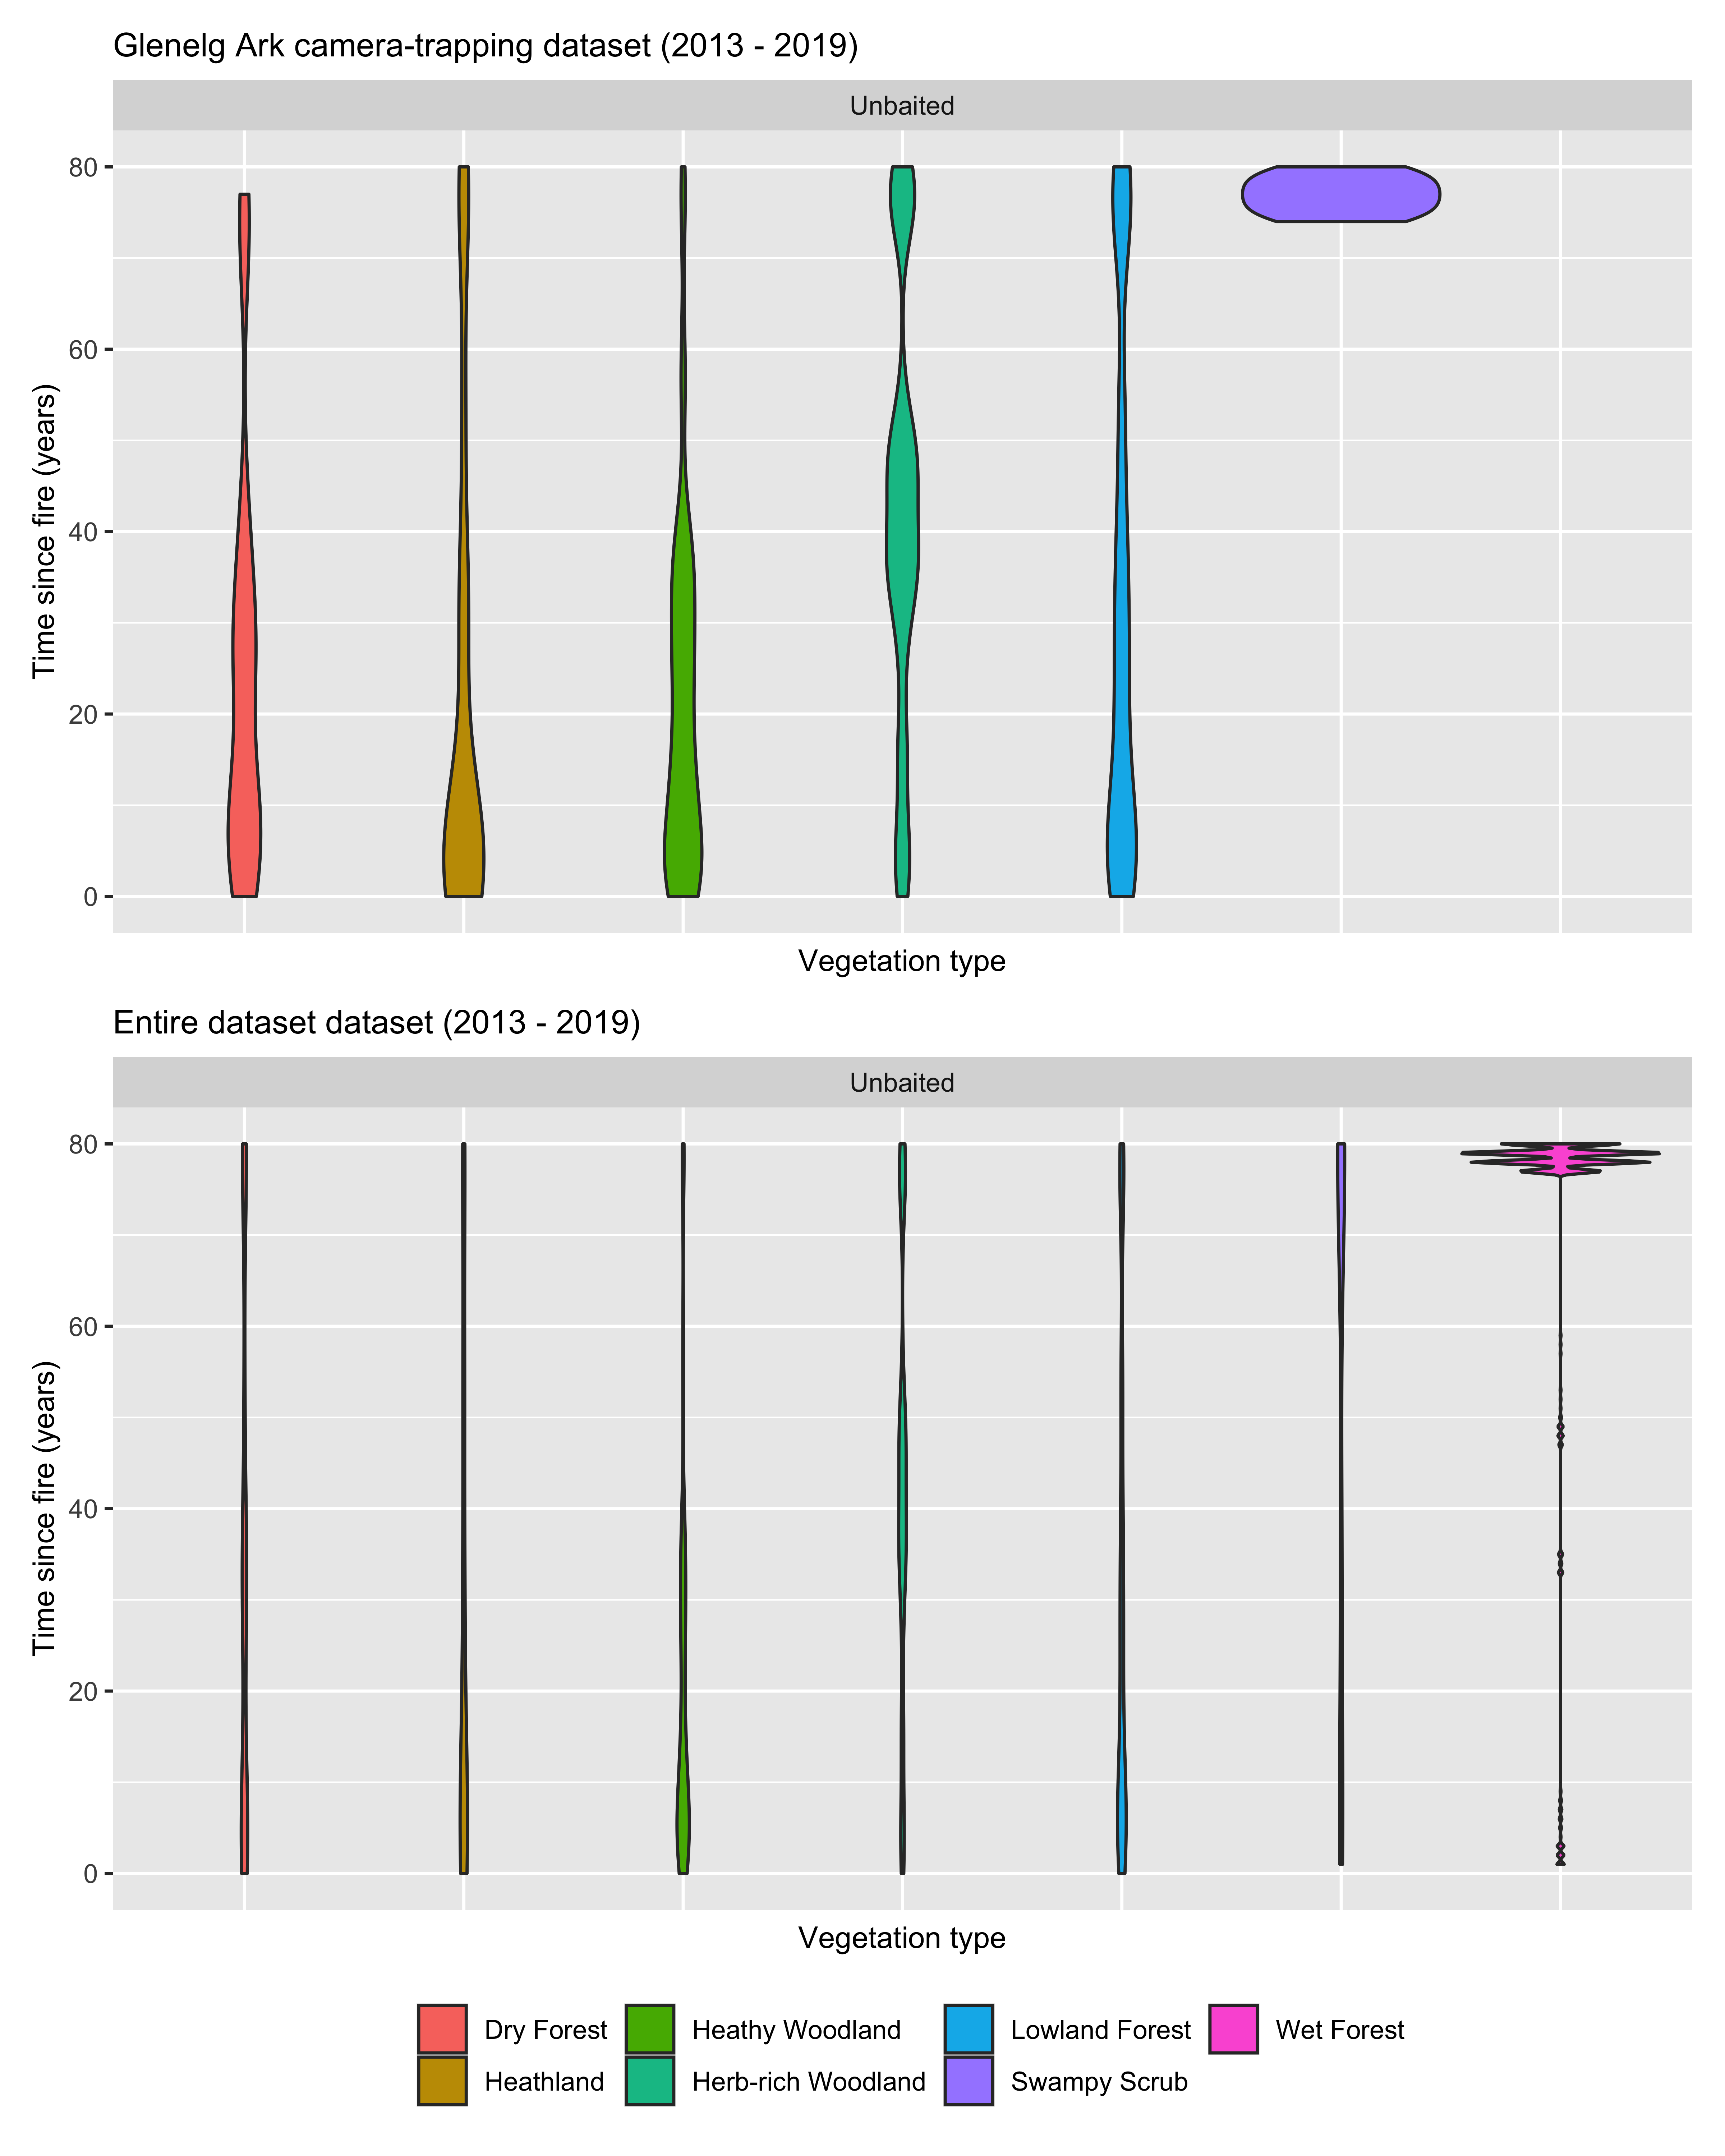
\includegraphics[width=0.8\linewidth]{../figs/raw_data_tsf_veg} 

}

\caption{Range and distribution of time since fire values across the surveyed vegetation types in baited and unbaited sites. In the Glenelg Ark camera-trapping dataset, where most sites in the baited landscapes are relatively recently burnt, and most sites are long-unburnt in the unbaited landscapes. Combining M.W.R PhD and Otway Ark surveys provides a wider range of fire history patterns in each vegetation type with and without fox control.}\label{fig:veg-tsf-violin}
\end{figure}

\newpage

\begin{figure}

{\centering 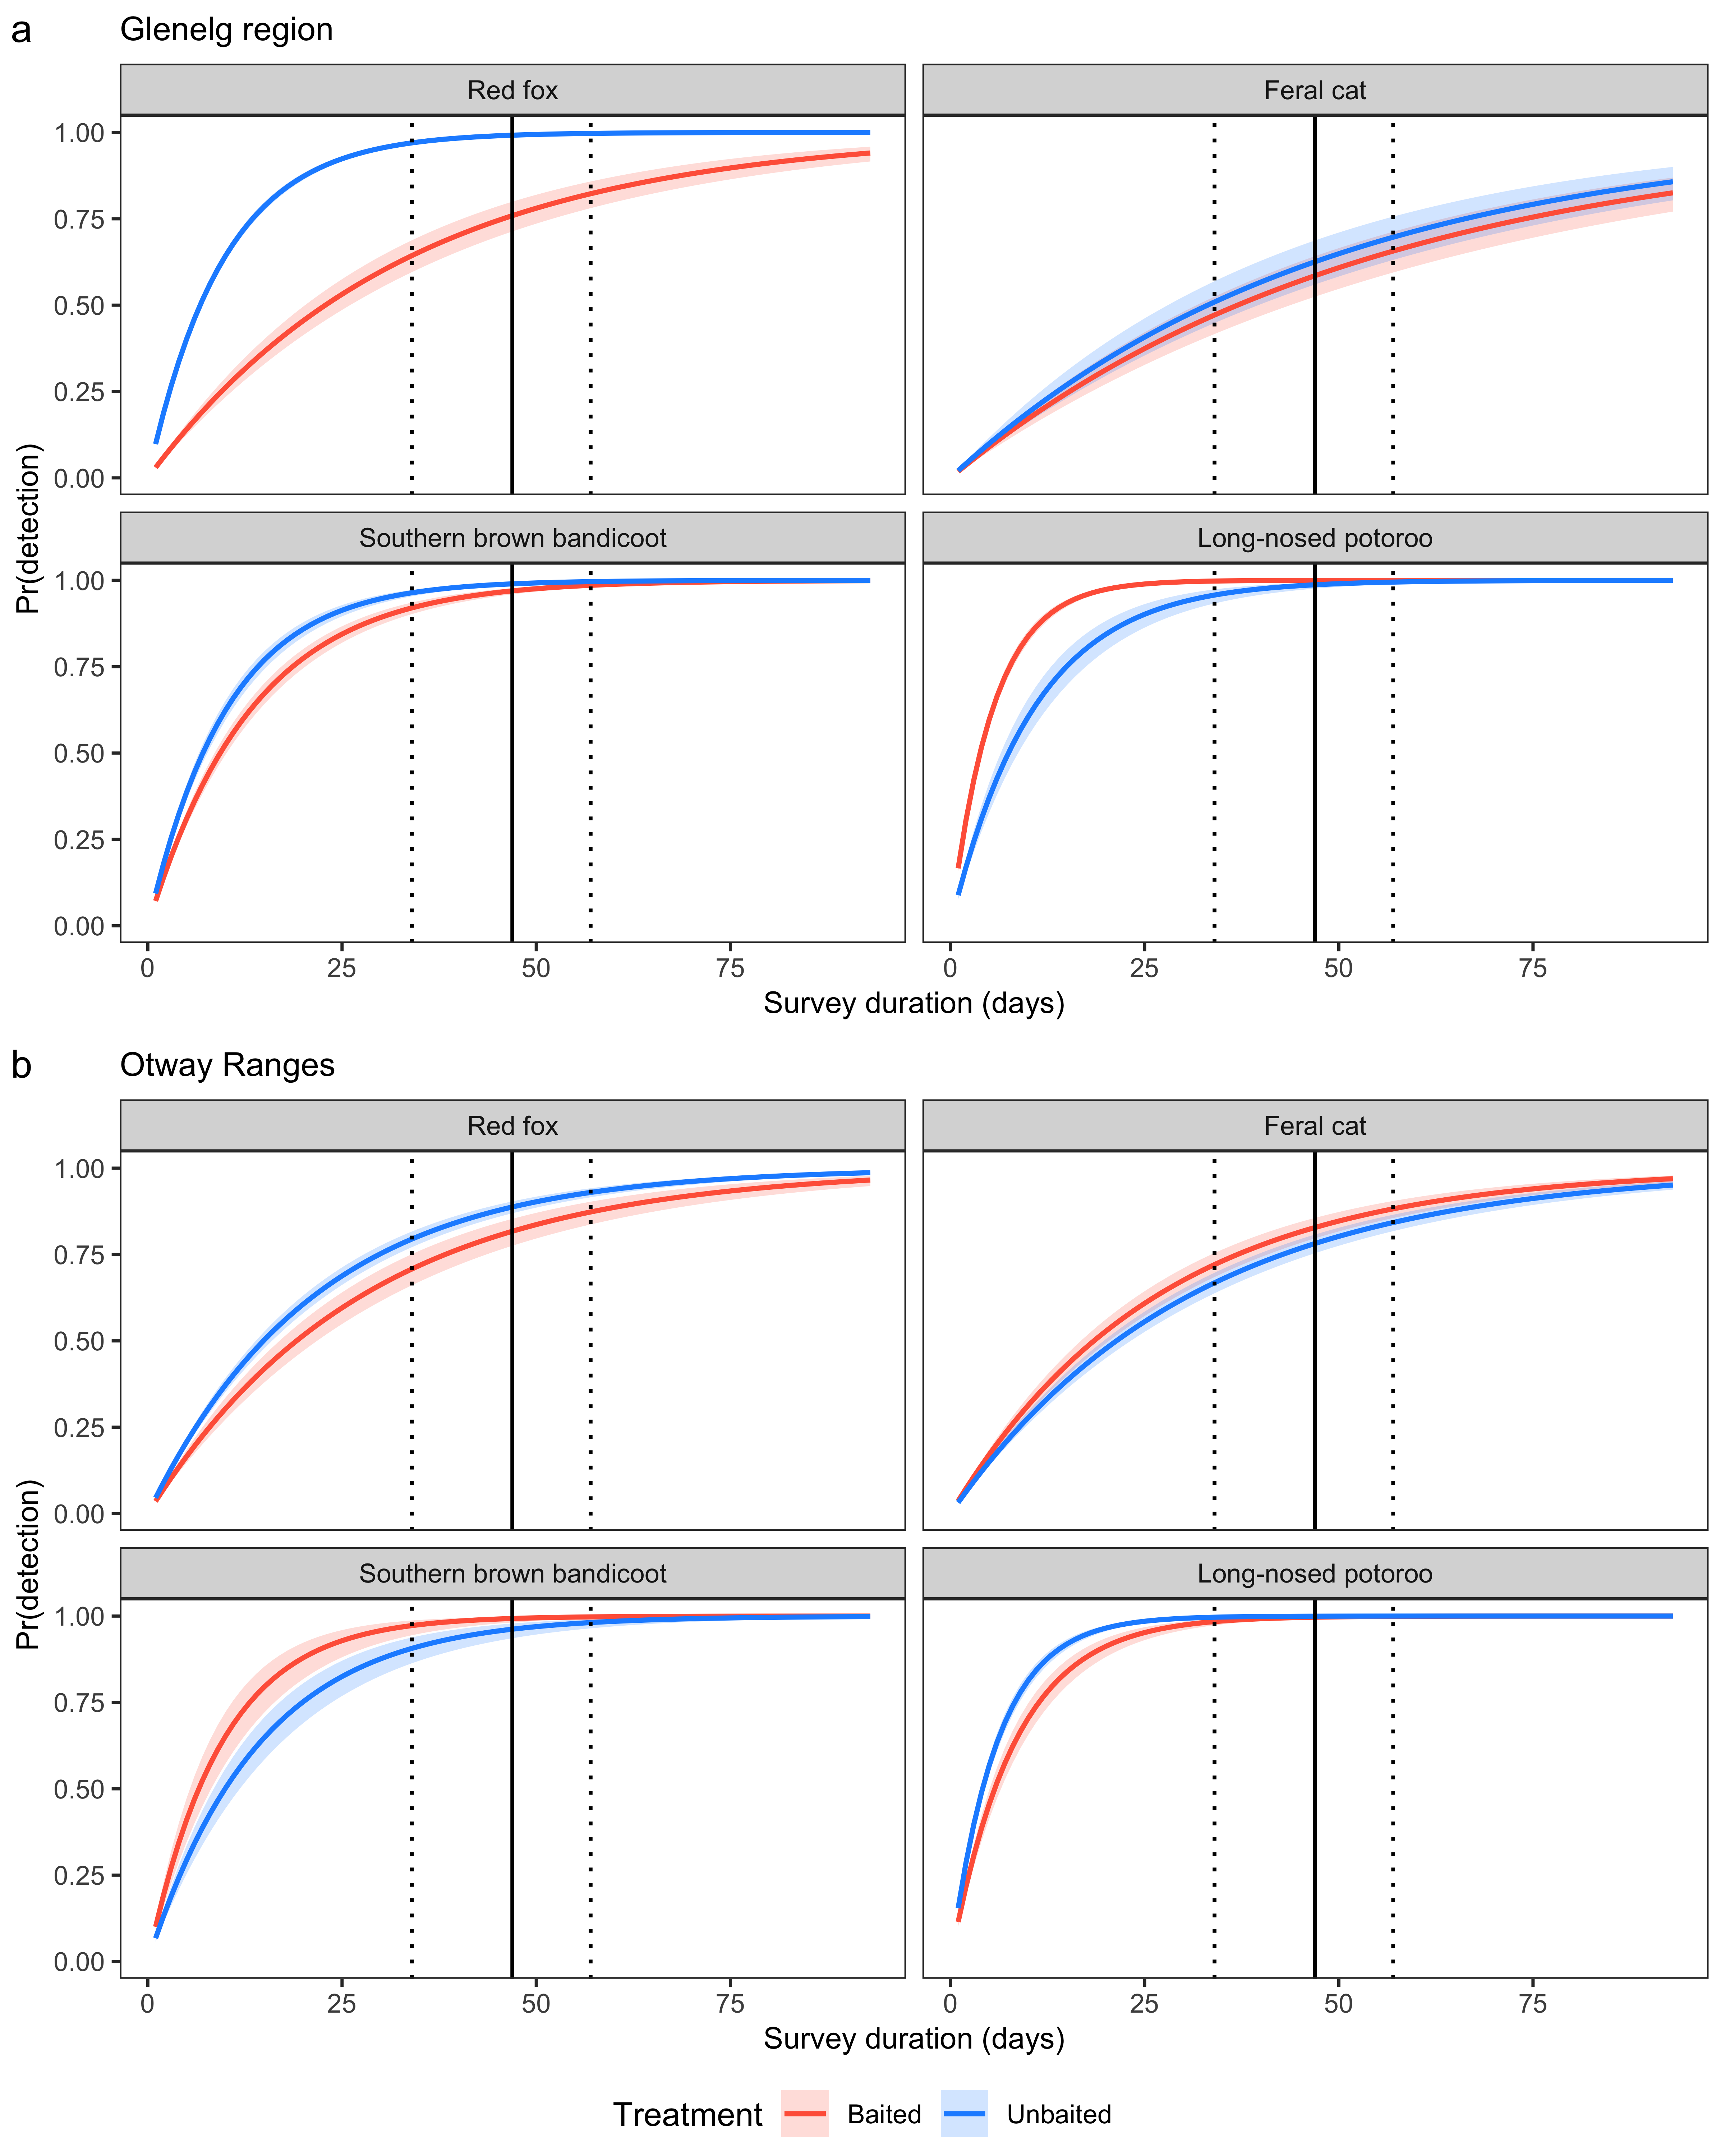
\includegraphics[width=0.8\linewidth]{../figs/detectability} 

}

\caption{Cumulative detection probabilities of species in landscapes with fox control (red) and without fox control (blue) in the Glenelg region (a) and Otway Ranges, south-west Victoria, Australia. Fox control had occurred in The Glenelg region for 8 - 13 years and was monitored with a control-impact design. The Otway Ranges was monitored using a before-after-control-impact experimental design; surveyed approximately 1 year prior and 2 years following the commencement of fox-baiting. Vertical grey lines represent mean (solid) as well as 25\% and 75\% quantiles (dotted) of days camera-traps were active for. Shaded bands represent 95\% Bayesian credible intervals. Estimates derived from Bayesian occupancy-detection models.}\label{fig:occ-cumdet}
\end{figure}

\newpage

\begingroup\fontsize{10}{12}\selectfont

\begin{longtable}[t]{lrrr}
\caption{\label{tab:occ-rain-aic}Akaike's Information Criterion values for generalised additive models with different rainfall periods.}\\
\toprule
Species & Months & AIC & dAIC\\
\midrule
Red fox & 6 & 4150.14 & 0.00\\
Red fox & 18 & 4151.57 & 1.43\\
Red fox & 24 & 4156.49 & 6.35\\
Red fox & 12 & 4158.20 & 8.06\\
Feral cat & 6 & 3732.68 & 0.00\\
\addlinespace
Feral cat & 12 & 3733.39 & 0.71\\
Feral cat & 18 & 3733.39 & 0.71\\
Feral cat & 24 & 3733.39 & 0.71\\
Southern brown bandicoot & 6 & 1868.55 & 0.00\\
Southern brown bandicoot & 24 & 1868.56 & 0.00\\
\addlinespace
Southern brown bandicoot & 18 & 1874.10 & 5.54\\
Southern brown bandicoot & 12 & 1877.49 & 8.94\\
Long-nosed potoroo & 12 & 1577.71 & 0.00\\
Long-nosed potoroo & 18 & 1581.19 & 3.48\\
Long-nosed potoroo & 24 & 1581.34 & 3.62\\
\addlinespace
Long-nosed potoroo & 6 & 1582.96 & 5.25\\
\bottomrule
\multicolumn{4}{l}{\rule{0pt}{1em}\textit{Note: }}\\
\multicolumn{4}{l}{\rule{0pt}{1em}AIC - Akaike's Information Criterion score}\\
\multicolumn{4}{l}{\rule{0pt}{1em}dAIC - difference between AIC of this model and the model with smallest AIC}\\
\end{longtable}
\endgroup{}

\newpage

\begingroup\fontsize{10}{12}\selectfont

\begin{longtable}[t]{llrrrr}
\caption{\label{tab:occ-model-sumstats}Generalised additive model summary statistics for models with 'full' set of explanatory variables relative to a 'null model' with only a site random effect.}\\
\toprule
Species & Model & EDF & dev.expl & r.sq & AIC\\
\midrule
Red fox & null & 420.65 & 0.28 & 0.27 & 4392.19\\
Red fox & full & 240.21 & 0.26 & 0.27 & 4150.14\\
Feral cat & null & 300.15 & 0.24 & 0.22 & 3901.10\\
Feral cat & full & 214.76 & 0.24 & 0.24 & 3732.68\\
Southern brown bandicoot & null & 242.65 & 0.36 & 0.27 & 2079.84\\
\addlinespace
Southern brown bandicoot & full & 185.37 & 0.40 & 0.32 & 1868.55\\
Long-nosed potoroo & null & 280.29 & 0.50 & 0.45 & 1671.09\\
Long-nosed potoroo & full & 256.45 & 0.53 & 0.47 & 1577.71\\
\bottomrule
\multicolumn{6}{l}{\rule{0pt}{1em}\textit{Note: }}\\
\multicolumn{6}{l}{\rule{0pt}{1em}EDF - estimated degrees of freedom of all model terms.}\\
\multicolumn{6}{l}{\rule{0pt}{1em}dev.expl - proportion of the null deviance explained by the model. }\\
\multicolumn{6}{l}{\rule{0pt}{1em}r.sq -  adjusted r-squared value.}\\
\multicolumn{6}{l}{\rule{0pt}{1em}AIC - Akaike's Information Criterion score}\\
\end{longtable}
\endgroup{}

\newpage

\begin{figure}

{\centering 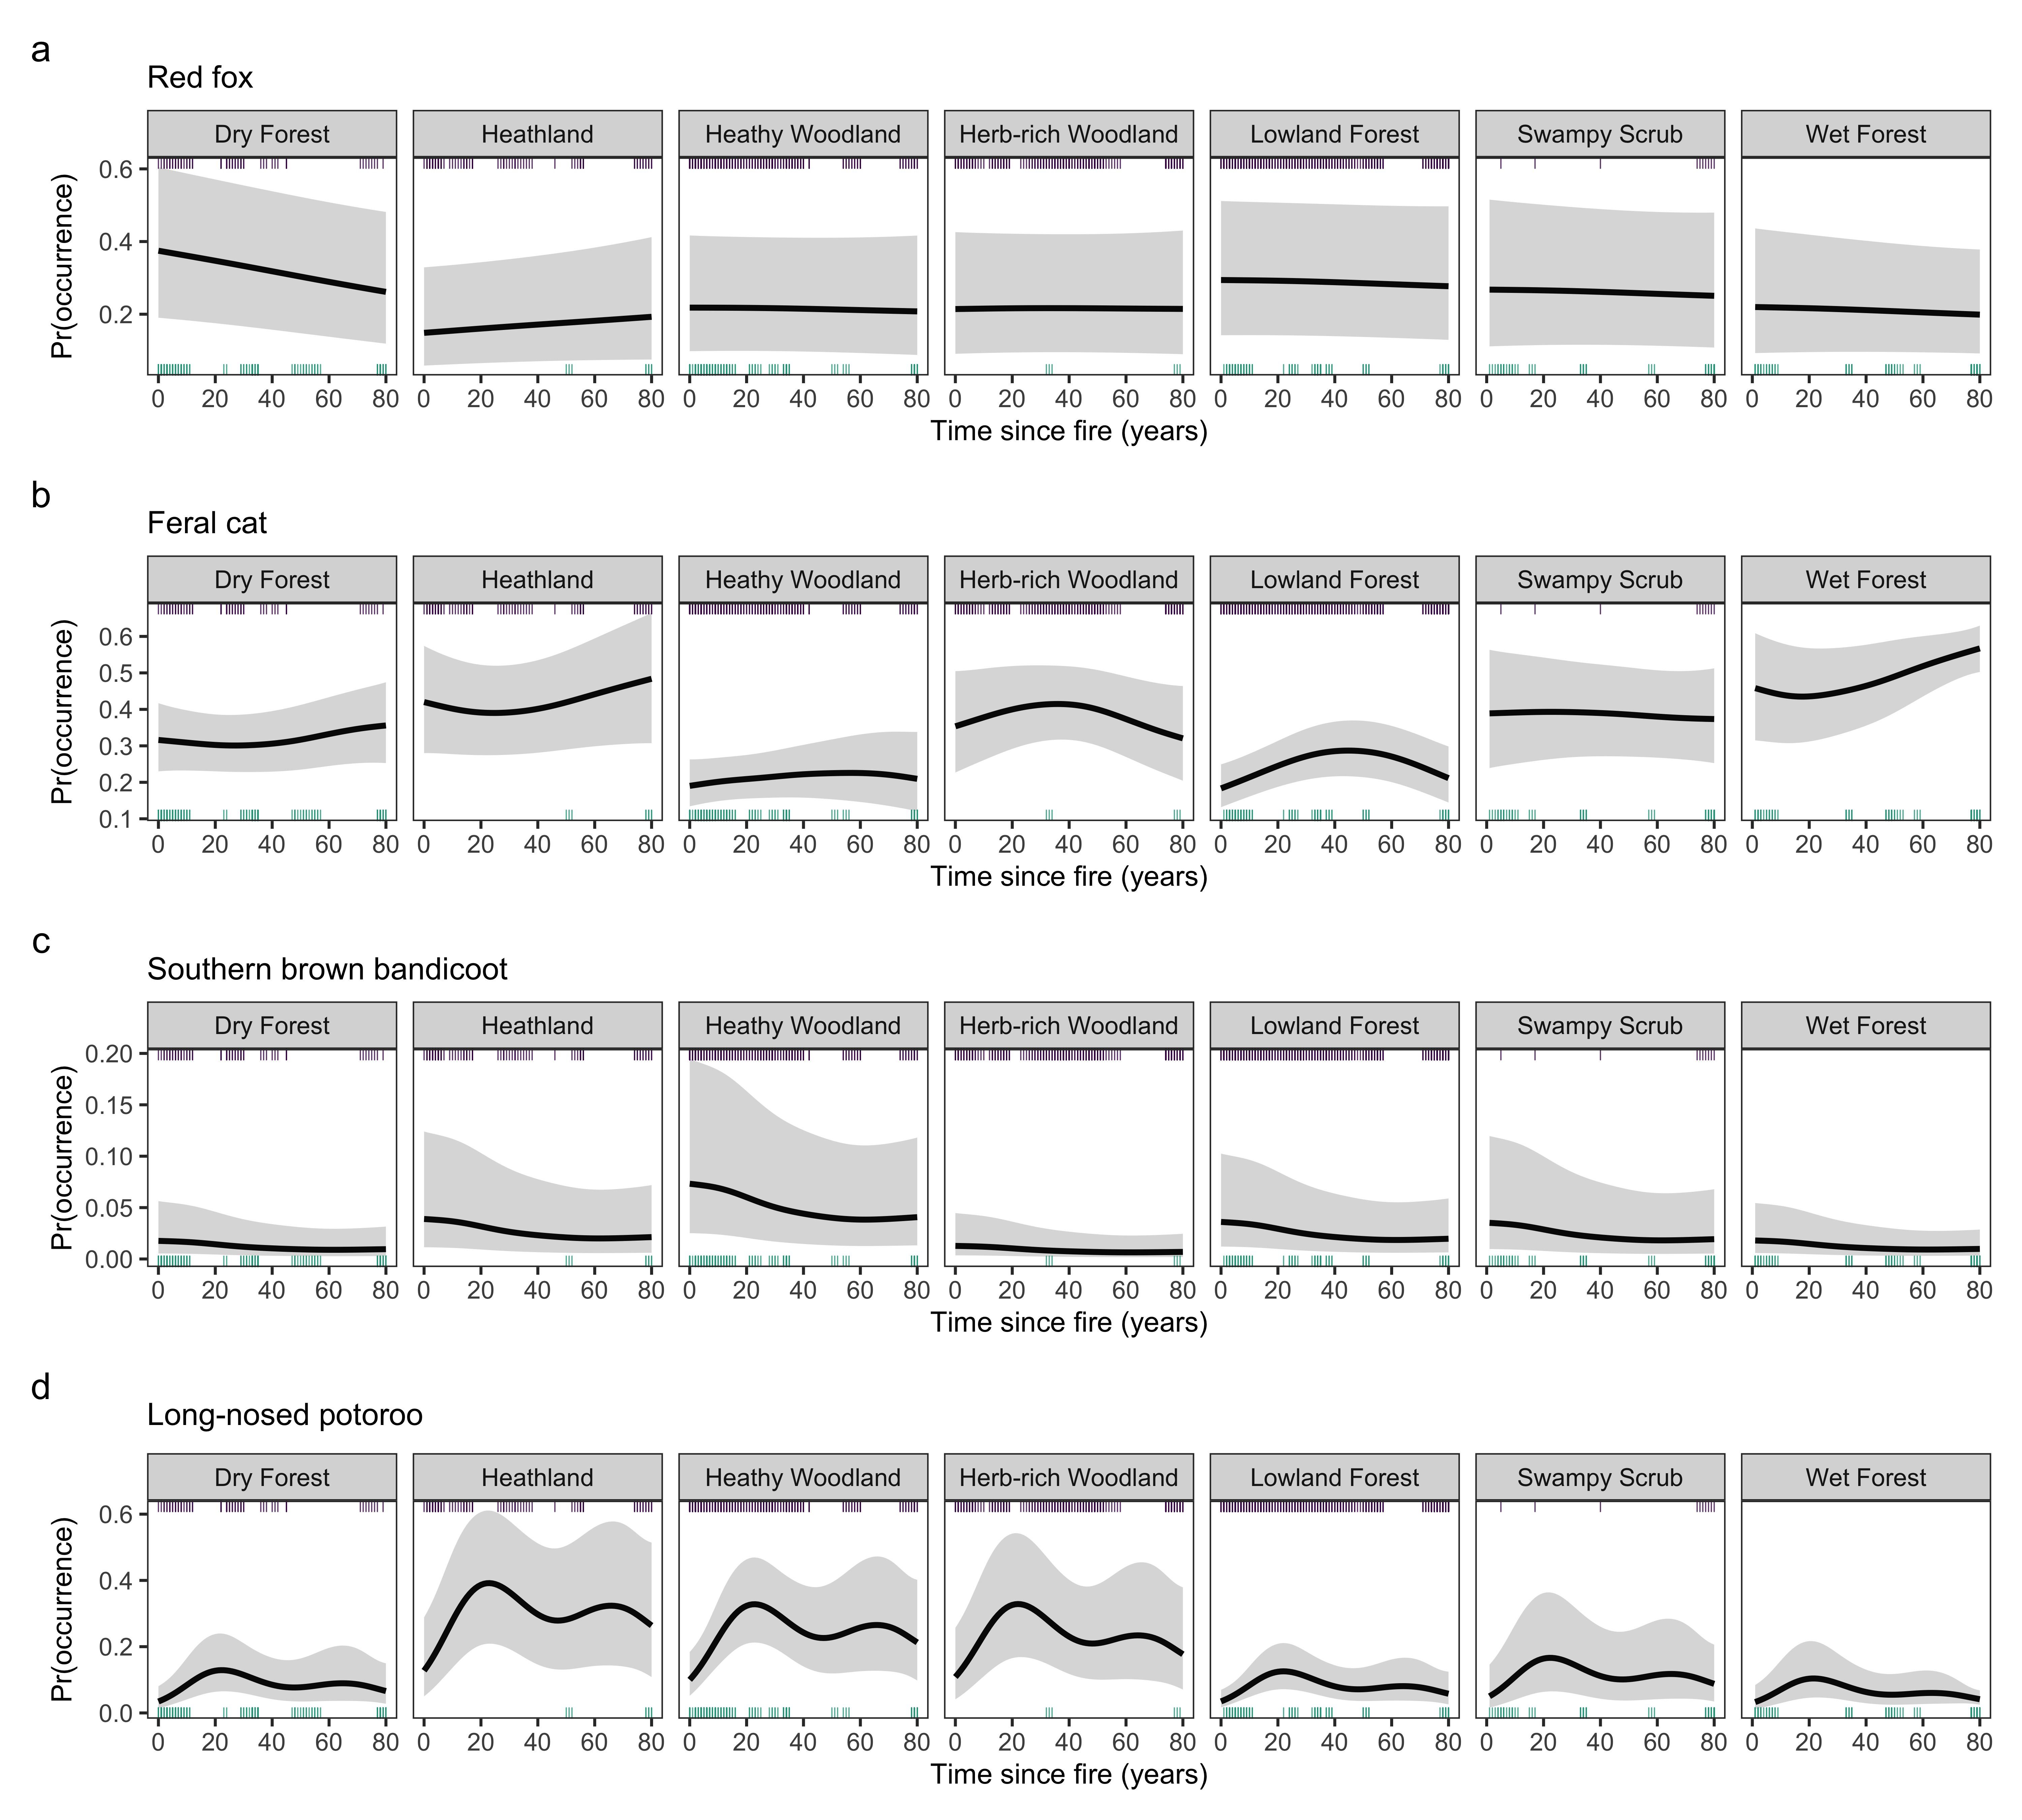
\includegraphics[width=0.8\linewidth]{../figs/tsf} 

}

\caption{Time since fire had a weak impact on fox (a) and feral cat (b) occupancy probability in south-west Victoria, Australia. Southern brown bandicoot occupancy probability (c) peaked around 15 and 75 years following fire, although, the magnitude of both peaks differed across Ecological Vegetation Class groups. Long-nosed potoroo occupancy probability (d) linearly increased with time since fire in heathy vegetation groups, but linearly decreased with years post-fire in Herb-Rich Woodlands. Estimates derived from generalised additive models (assuming perfect detection). Shaded regions indicate 95\% confidence intervals. Rug ticks representing the distribution of time since fire data for the Glenelg region (brown) is shown on the inside of the top axis, Otway Ranges distribution shown on the inside of the bottom axis (navy).}\label{fig:occ-tsf}
\end{figure}


\end{document}


